\documentclass[a4paper,11pt]{kth-mag}
\usepackage[T1]{fontenc}
\usepackage{textcomp}
\usepackage{lmodern}
\usepackage{amsmath}
\usepackage[latin1]{inputenc}
\usepackage[swedish,english]{babel}
\usepackage{enumitem}% http://ctan.org/pkg/enumitem
\usepackage[toc,page]{appendix}
\usepackage{graphicx}
\usepackage{xcolor}
\usepackage{listings}
\usepackage{attachfile}
\usepackage{color}

\definecolor{dkgreen}{rgb}{0,0.6,0}
\definecolor{gray}{rgb}{0.5,0.5,0.5}
\definecolor{mauve}{rgb}{0.58,0,0.82}

\lstset{frame=tb,
  language=[Sharp]C,
  aboveskip=3mm,
  belowskip=3mm,
  showstringspaces=false,
  columns=flexible,
  basicstyle={\small\ttfamily},
  numbers=none,
  numberstyle=\tiny\color{gray},
  keywordstyle=\color{blue},
  commentstyle=\color{dkgreen},
  stringstyle=\color{mauve},
  breaklines=true,
  breakatwhitespace=true,
  tabsize=3
}
\graphicspath{{Pics/}}
\usepackage{modifications}


\title{A comparison of visualisation techniques for complex networks}

\subtitle{En j\"amf\"orelse av visualiseringsmetoder f\"or komplexa n\"atverk}
\author{Viktor Gummesson\\ \lowercase{vgum@kth.se}}
\blurb{Master's Thesis in Computer Science\\Royal Institute of Technology\\[5pt]Supervisor, KTH: Olov Engwall\\Examiner: \selectlanguage{Swedish} Olle B\"{a}lter\\Project commissioned by: Scania\\Supervisor at Scania: Magnus Kylleg\aa rd}

\begin{document}
\frontmatter
\pagestyle{empty}
\removepagenumbers
\maketitle
\selectlanguage{english}
\begin{abstract}
The need to visualise big sets of data and networks within a company is a well-known task. In this thesis, research has been done of techniques used to visualize complex networks in order to find out if there is a 
generalized optimal technique that can visualize complex networks.

For this purpose an application was implemented containing three different views, that were selected from the research done on the subject. As it turns out, it points toward that there is no generalized optimal 
technique which can be used to default visualize complex networks in a satisfactory way. A definit conclusion could not be given due to the fact that all visualization techniques which excist could not be
evaluated within this thesis timeframe.
\end{abstract}
\clearpage
\begin{foreignabstract}{swedish}
Behov av att visualisera data inom bolag \"ar ett k\"ant faktum, denna avhandling har anv\"ant olika tekniker f\"or att unders\"oka om det existerar en generell optimal teknik som kan till\"ampas vid visualisering av komplexa n\"atverk.
 Vid genomf\"orandet implementerades en applikation med tre olika vyer, de valdes ut baserat p\aa \space forskning inom det valda omr\aa det. Resultatet visade att det inte existerar en generell optimal teknik som kan till\"ampas vid
 visualisering av komplexa n\"atverk, det medf\"or att en definitiv slutsats inte uppn\aa s. Det p\aa \space grund av att alla de visualiseringstekniker som existerar inte kunde unders\"okas inom avhandlingens tidram.
\end{foreignabstract}
\clearpage
\tableofcontents*
\mainmatter
\pagestyle{newchap}
\chapter{Introduction}
This chapter is intended to give an introduction to the subject of visualizing networks.
\section{Background}
To be able to visualize different networks is an important part in many fields, such as science and technology. For example, computer science that deals with complex networks of relationships between system components,
displaying relations in a social network, molecular biology that study the interactions between various systems of cells, e.t.c.

There are different approaches to take when visualizing networks. The most traditional approach is to represent the network as some kind of graph, because many structures in different scientific fields can be represented
as a node-link graphs. Where nodes represents different components which are visualized with a shape and edges represents different components relations which are visualized by a connecting line between two nodes.

\section{Arising problems with growing data}
Though the traditional ways of visualizing graphs are pleasing and give an intuitive way of looking at relations, there are problems which can arise when the networks that needs to be visualized are of a larger size. The traditional
way may be sufficient when dealing with networks of small sizes of nodes and relations, but what will happen when the networks become complex and have hundreds or thousands of nodes?
\subsection{Edge and node crossing}
When the node count becomes larger, the area dedicated to layout these nodes becomes smaller. This can contribute to nodes starting to overlap each other, making it hard to distinguish between a set of different nodes.

A similar problem arises concerning edges. Depending on the layout of the nodes a different amount of edges may overlap, crossing each other. This may not be a problem if the number of crossings is low or the angle between 
two edges is high. But when this angle decreases and the number of crossings increases it becomes harder to distinguish between specific edges, to see which edge connects to which node. If the relations are of a large enough size the cluster of edges
may become one big black area.

When dealing with layout techniques one strives to layout the nodes in a way that minimize node- and edge crossings.
\subsection{Labeling}
Labeling nodes and edges in a network become more challenging as the network grows. In fact the optimal label placement of a graph has been shown to be NP-Complete\cite{Marks91thecomputational}.
The task of labeling can be divided into three different labeling tasks:
\begin{itemize}
	\item{Labeling area features (clusters).}
	\item{Labeling line features (edges).}
	\item{Labeling point features (nodes).}
\end{itemize}
\subsection{Situation awareness}
Human and psychology factors play a role when visualizing a network, situation awareness is a term in this aspect. Endsley\cite{195097} defines situation awareness as:
\begin{quote}
\emph{Situation Awareness is the perception of the elements in the environment within a volume of time and space, the comprehension of their meaning, and
the projection of their status into the near future}
\end{quote}
Situation awareness becomes important to consider when choosing visualisation technique.

Figure \ref{fig:hair_ball} shows  what can happen when trying to visualize big networks.

\newpage
\begin{figure}[!htbp]
	\centering
	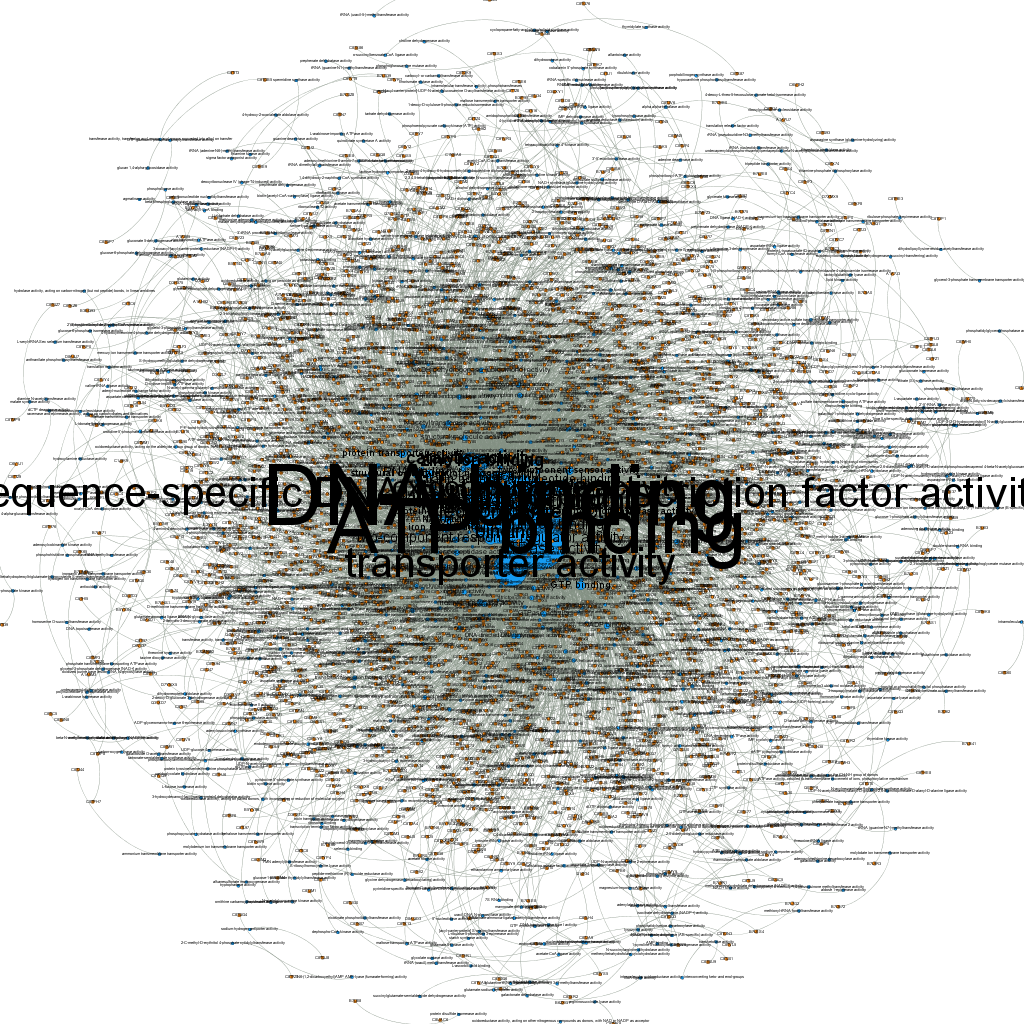
\includegraphics[scale=0.4]{HairBallGraph}
	\caption{Example of a graph where the problem of node- and edge crossing becomes obvious}
	\label{fig:hair_ball}
\end{figure}
\newpage
\section{This thesis}
This thesis revolves around the question:\\
\\
\emph{Which types of visualization techniques are suitable for visualizing large and complex networks?}\\
\\
With the corresponding hypothesis that:\\
\\
\emph{One can conclude that some visualization techniques are better suited than others and that one or several may be best for the task at hand.}
\\

In chapter two different common visualisation techniques are described. Chapter three goes through the methodology used to evaluate a set of different techniques. Chapter four provides the results from chapter 3. Chapter five discusses
the results and conclusions.
\chapter{Visualization techniques and their theory}
\label{Theory}
There exist a number of different approaches and techniques used to visualize large and complex networks. This chapter is intended to introduce some of these and explain how they work.
\section{Fundamental techniques}
Though there exist a number of different approaches many of these are based on some fundamental technique or concept. Two major aspects are important to consider when trying to visualize a network. First is about the part that
most probably relate to graph visualization, the actual layout algorithm that decides where each node is to be placed and how the edge routing is made. Second is the aspect of how one is to navigate a graph when it has been
generated, that is navigation such as zooming and panning.
\subsection{Force-Directed}
Force-directed is a popular class for a type of algorithm for calculating layouts of graphs. They are constructed to strive towards generating graphs with node positions so that edges in the graph are of equal length and the layout
displays as much symmetry as possible. One of the pros with these algorithms is that they are flexible, they do not rely on domain specific knowledge but instead only use the information contained within the structure of the graph. Graphs produced
by these algorithms tend to be aesthetically pleasing and exhibit symmetries\cite{1338}. Figure \ref{fig:force_directed_ex1} shows an example of a graph drawn with a force-directed algorithm.

\begin{figure}[!htbp]
	\centering
	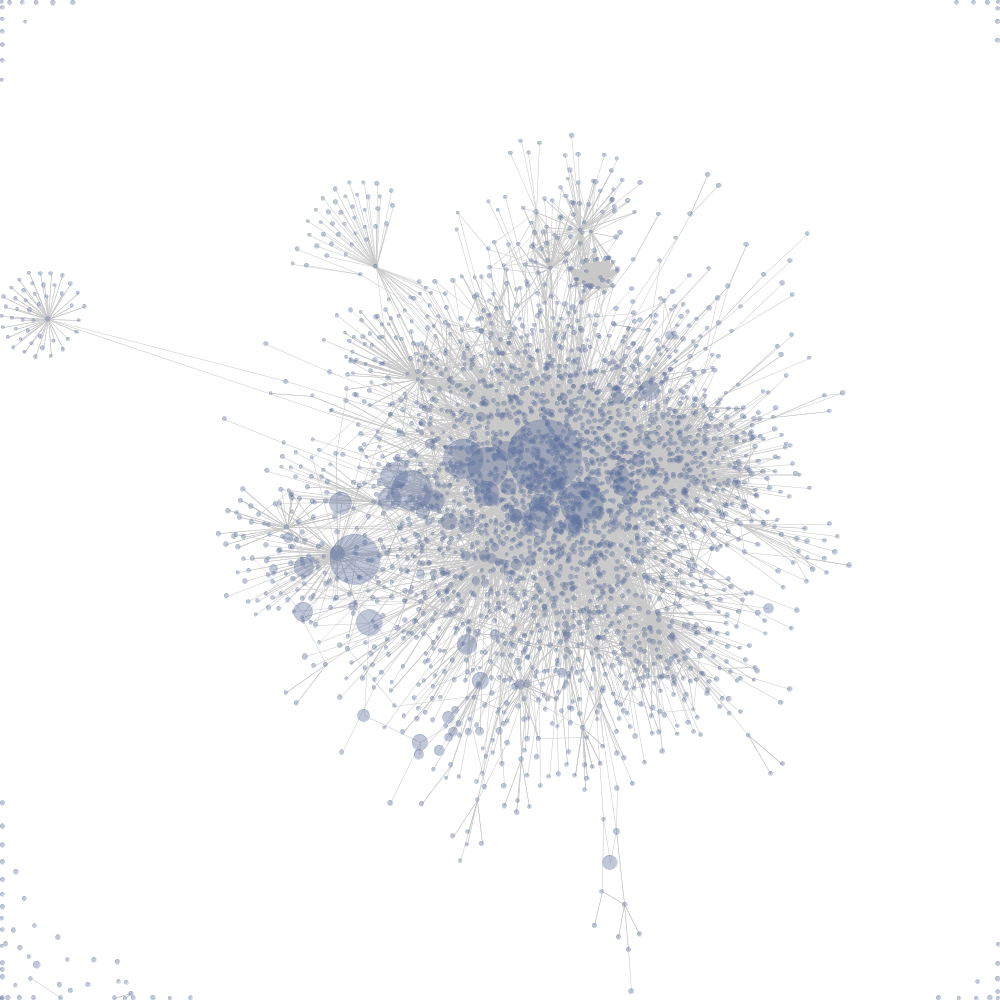
\includegraphics[scale=0.3]{ForceDirectedEx1}
	\caption{Visualization of links between pages on a wiki using a force-directed layout.}
	\label{fig:force_directed_ex1}
\end{figure}

These algorithms are based on assigning forces between nodes and edges in a graph, simulating the motion of the edges and nodes or minimize their energy. One of the first force-directed algorithm dates back to 1963 with 
the algorithm of Tutte\cite{tutteFD} and is based on barycentric representation\cite{1338}. Though the more commonly used algorithms such as Eades\cite{ead} and Fruchterman and Reingold\cite{fr} both rely on spring forces similar to those in
Hooke's law. Here there are repulsive forces between all the nodes in a graph while in the same time attractive forces between nodes and their neighbours. As in the Eades algorithm \cite{1338} where
they have an initial random layout of nodes. Having nodes represented as steel strings and edges as springs. Then letting the system move towards a state where minimal energy between 
nodes are achieved.

Besides striving towards equal edge length and displaying symmetry one can argue that the graph layout also should strive to have an even vertex distribution for a more pleasing layout. The algorithm of Fruchterman and Reingold
cover this by using a bit of a different physical model, seeing the vertices in a graph as atomic particles or as celestial bodies. Where the attractive forces are defined as \cite{1338}:\\
\begin{mathsurround}
\\
\math f_{a}(d)=\frac{d^2}{k}\\
\\
\end{mathsurround}
 Repuslive as:\\
\begin{mathsurround}
\\
\emph{\math f_{r}(d)=\frac{-k^2}{d}}
\\
\end{mathsurround}
Where d is the actual distance between two vertices and k is the optimal distance. K is defined as:\\
\begin{mathsurround}
\\
\emph{\math k=C\sqrt{\frac{area}{number of vertices}}}
\\
\end{mathsurround}

Besides from this the algorithm also uses the notion of temperature as a refining step. This works so that when the algorithm improves the layout the adjustments become smaller from the last iteration of the algorithm.
 
As the graph size grows larger, graphs with more than a few hundred vertices, a problem arises with the basic force-directed algorithms. The fact is that the used physical model has multiple local minima, and a graph produced
with only a local minima can be much worse than would it be produced with the global minima. Algorithms have been developed trying to avoid local minima, such as the Hadany and Harel algorithm \cite{handh}, which is based on
a multi-level layout technique that works with graphs containing 15000 vertices. 

In multi-level techniques the graph structure that is to be drawn is viewed in substructures where each substructure has less complexity then the whole. These substructures are then laid out in order from the most simple 
structure to the most complex one. Hadany and Halers \cite{handh} said it good as that a natural strategy for drawing a graph in a pleasant manner is to first consider an abstraction, 
disregarding some of the graphs fine details. Afterward add details to correct the layout. They also take up the importance of preserving the essential features of the graph in the abstraction,
so it becomes of importance to be able to point out the essential feature of a graph. 

\subsection{Navigation through zooming}
The way one zooms becomes a large part when navigating a graph, how one does this greatly affects the situational awareness. When navigating through a graph both global context and local details are of importance. Global context
is provided when one can navigate through a graph and still be able to orient oneself according to the graph. Which most often requires one to be far zoomed out to see the whole. Though when zoomed out the local details are not 
on a high enough level to give any real information. So to get out more detailed information one is needed to zoom in the graph to a specific area, which is when a tunnel vision problem arises. 
Causing one to easier lose orientation and information of the overall dependencies when the context is lost.

FishEye view is a technique that address this problem of tunnel vision. One can compare the technique to a fisheye lens used by cameras for the creation of wide panoramic images. The techniques allows one to show high detail
at focus while displaying less and less detail about information that are further away from focus, how much depends on how far away it lies. Figure \ref{fig:FishEye} shows an example of this. Extra effective this becomes if the data one works with has a clear structure so
that one can cluster this data.

\begin{figure}[!htbp]
	\centering
	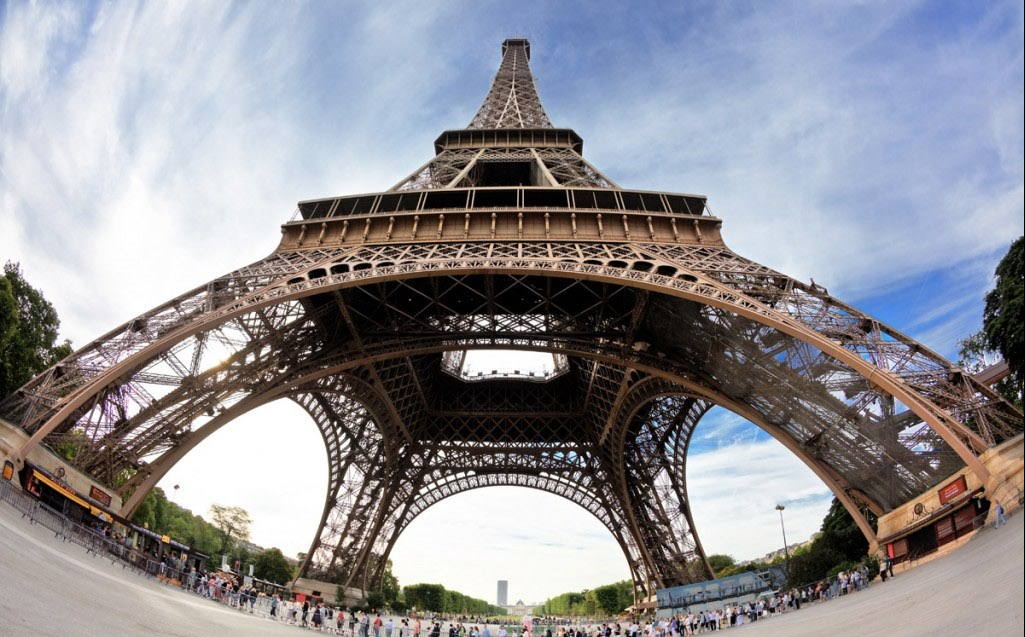
\includegraphics[scale=0.3]{FishEyeEiffel}
	\caption{Picture of the Eiffel Tower displaying the fisheye effect. Here the base of the tower is in focus, showing details of the base while still having the whole tower in the picture.}
	\label{fig:FishEye}
\end{figure}

\cite{Schaffer:1996:NHC:230562.230577} used the FishEye method while navigating networks where nodes was represented by squares and  
nodes did not overlapp each other. The data used was clustered in a way that one node could contain a subset of different nodes. Figure \ref{fig:FishEyeCluster} shows an example of such a graph and a 
possible clustering of it.

\begin{figure}[!htbp]
	\centering
	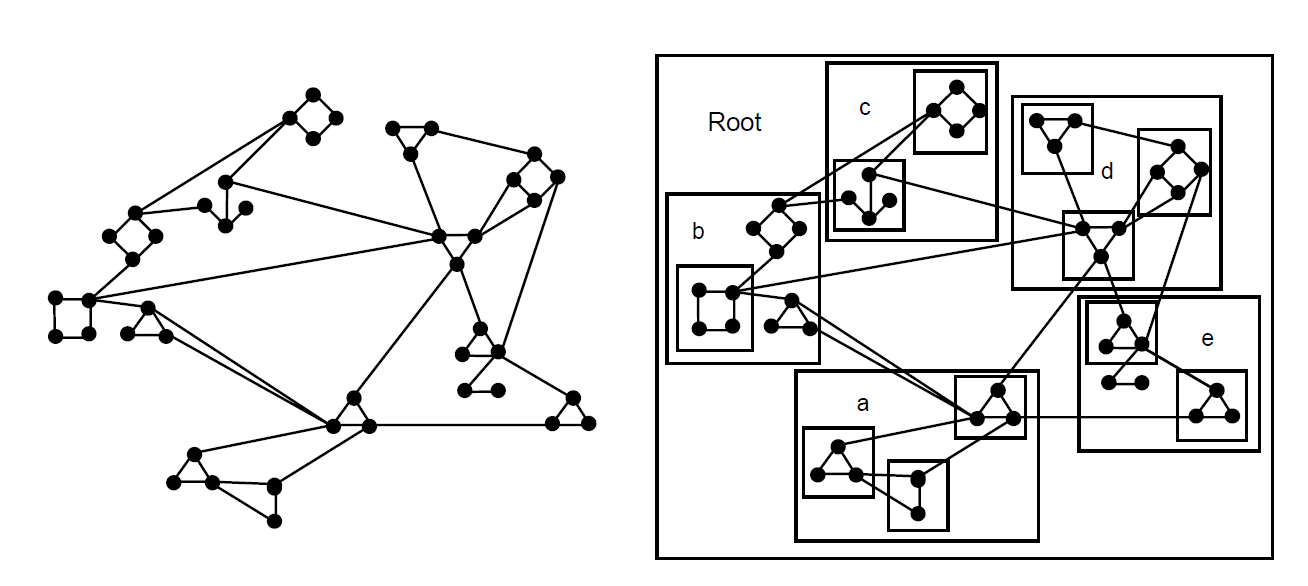
\includegraphics[scale=0.3]{FishEyeCluster}
	\caption{Graph that are divided into clusters.}
	\label{fig:FishEyeCluster}
\end{figure}

When zooming one actually zooms a node/nodes (cluster/clusters). This translate into the FishEye view where the zoomied node/nodes are in focus, getting larger, and the
other node/nodes being outside focus are getting shrunken. Figure \ref{fig:FishEyeZoom} shows an example of a graph before a zooming action and after.

\begin{figure}[!htbp]
	\centering
	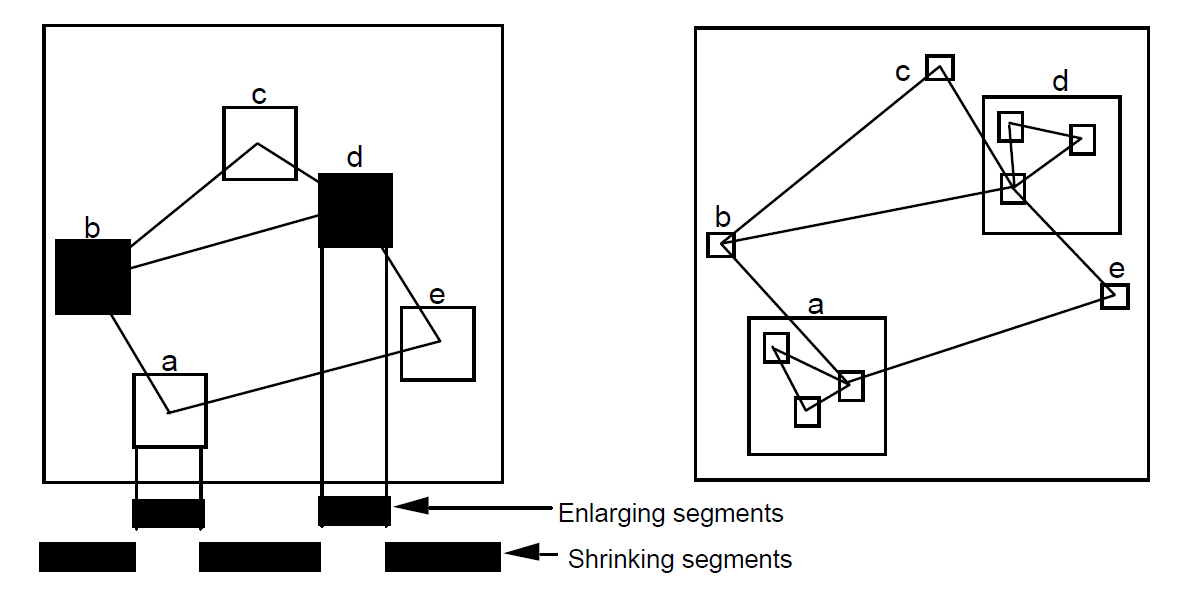
\includegraphics[scale=0.3]{FishEyeZoom}
	\caption{Example of graph when zoomed (element b and a selected for zooming). Left hand side shows the graph before zooming and which segments are being enlarge and which are being shrunken. Right hand side shows the graph after zooming.}
	\label{fig:FishEyeZoom}
\end{figure}
\newpage
\section{Two-dimensional space}
This chapter introduce methods used to visualize large networks in a two-dimensional space. One benefit when using a layout in 
the two-dimensional space is that one can get away from the problem of nodes concealing each other. 
\subsection{BioFabric}
BioFabric\cite{23102059} is a method that uses a different approach to represent a graph than the traditional way where one represents nodes
as a shape, like a circle or a rectangle, and edges as lines between nodes. Instead nodes are represented as one-dimensional
horizontal lines and edges as one-dimensional vertical lines. These vertical lines start at one of the horizontal lines (one specific node)
and end at another, representing a connection between these lines (nodes). This different approach lets one get away from the problem of node and edge crossings.
It guarantees no edge overlapping and no node overlapping.

A difficulty that can arise with many methods is when one handles updates of graphs, which can result in major alterations of a graphs layout when only a few nodes are introduced. 
This problem exists in BioFabric as well, but because of adding one node is the same as adding one horizontal line and adding a edge equal to adding a vertical line this can 
help to not having such a big affect on the graphs appearance. Though how much it alters the graph is dependent on how many nodes are added and how many connections to other nodes are
added.

As for how to layout the node and edges there are different approaches one can take. One basic approach is to do a breadth first traversal of the data to be displayed, where neighbouring nodes
are visited in the order determined by their degree (the data are structured by degree of nodes). Next follows an example of a way of assigning nodes and edges that uses this approach \cite{23102059}.
\\
\\
Node assignment:
\begin{enumerate}
	\item Set row 1 as the next available row.
	\item Find the highest degree node not yet processed, and
		  assign it to the next available row. Make that row the
		  current row; increment the next available row.
	\item Take the node assigned to the current row and
		  order its neighbours based upon their degree, highest
		  degree first.
	\item Traversing the neighbour nodes using that order, if the
		  node has not yet been assigned, assign it to the next
		  available row and increment the next available row.
	\item Increment the current row. If a node has been assigned
		  to that row, go to step 3. If not, go to step 2.
\end{enumerate}
\\
\\
Edge assignment:
\begin{enumerate}
	\item Set column 1 as the next available column. Make row
		  1 the current row c.
	\item For current row c, get all the unassigned edges for the
		  node in that row. Note that since we are not dealing
		  with shadow links, all unassigned edges must connect
		  to rows \begin{mathsurround} \math \ge \end{mathsurround} c.
	\item For each row r \begin{mathsurround} \math \ge \end{mathsurround} c, create a set S of edges incident on
		  c and r. Order these sets by increasing row number r,
		  so that edges will be assigned in order of increasing
		  length.
	\item Iterating through the ordered list of sets, for each set
		  S, order those edges in S based on lexicographic
		  ordering of the link relation description, and assign
		  them to the next available columns in this order;
		  increment next available column appropriately. If
		  there is a pair of directed edges with the same link
		  relation description, downward links are assigned
		  before upward links.
	\item Increment the current row, and go to step 2.
\end{enumerate}

Figure \ref{fig:bio_default} is an example of a big network visualized with BioFabric using the basic approach.

\begin{figure}[!htbp]
	\centering
	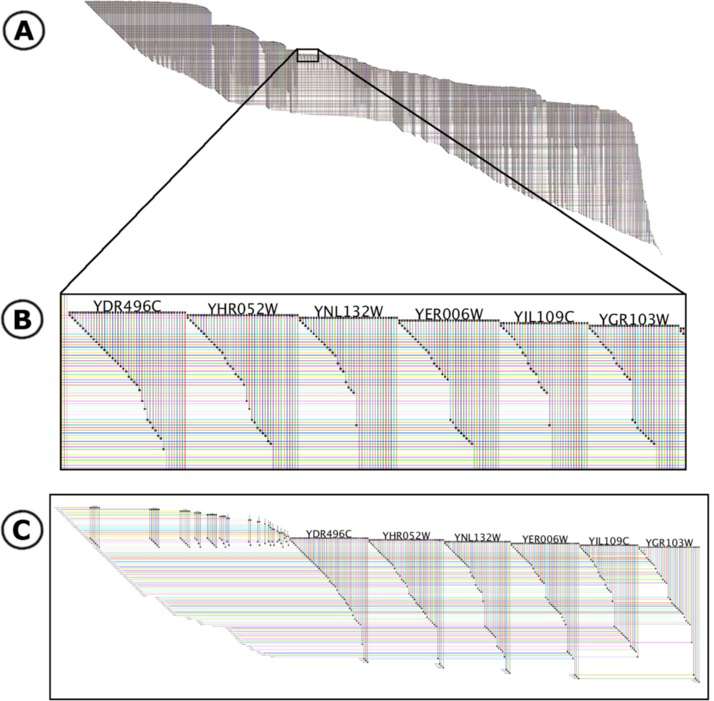
\includegraphics[scale=0.7]{BIODefault}
	\caption{This is a depiction of the yeastHighQuality.sif data set [3-5] containing over 3000 nodes and 6,800 edges.
The key feature of the BioFabric presentation is that nodes are depicted as horizontal lines, one per row; edges are presented as vertical lines,
each arranged in a unique column. Note how the use of darker colors for rendering edges and lighter colors for rendering nodes insures that the
former stand out despite the crossover. A) The view of the full network, laid out with the default algorithm. B) Detail of network shown boxed in
network A, which highlights one advantage of the BioFabric presentation technique: similarities, and differences, in the connectivity of different
nodes are immediately apparent. C) The six nodes and first neighbours depicted in a subset view, where all extra space has been squeezed out,
creating a compact presentation that still retains all the relative positioning from the full view. Note how the full inventory of edges incident on
the six nodes also includes those on the left originating from higher node rows.}
	\label{fig:bio_default}
\end{figure}


Other approaches that can be used are to try to group nodes based on similarity and difference between their connectivity. The way to
represent similarity could be to use cosine similarity\cite{website:Wikipedia} or Jaccard similarity\cite{website:Wikipedia2}. Figure \ref{fig:bio_sim} shows a network visualized 
using similarity weights, resulting in a less compact layout than the basic approach.

BioFabric has one release which is an open-source Java application with some documentation that can be found at\cite{website:biofabricdoc}. Though BioFabric is built on a relatively easy and intuitive algorithm, one could
take the option of implementing an own version. Having their own customized features that suits one's purpose.
\\


\begin{figure}[!htbp]
	\centering
	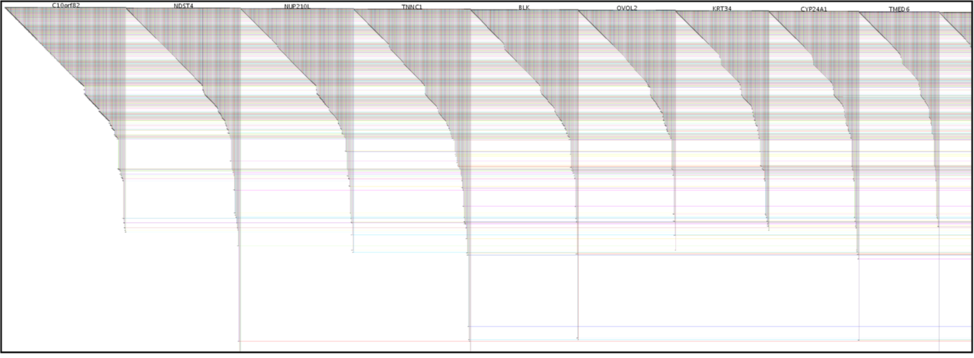
\includegraphics[scale=0.5]{BIOSim}
	\caption{Layout that tries to place nodes with similar connectivity next to each other in the linear ordering of nodes.}
	\label{fig:bio_sim}
\end{figure}

\subsection{HivePlots}
HivePlots is a visualisation algorithm that uses a number of radially oriented linear axis that have a coordinate system that is based on nodes properties. A networks nodes are layed out on these axes. Connecting nodes are
shown with edges between them, visualized as curves between nodes. Figure \ref{fig:hive_plot} shows an example of a HivePlot.

\begin{figure}[!htbp]
	\centering
	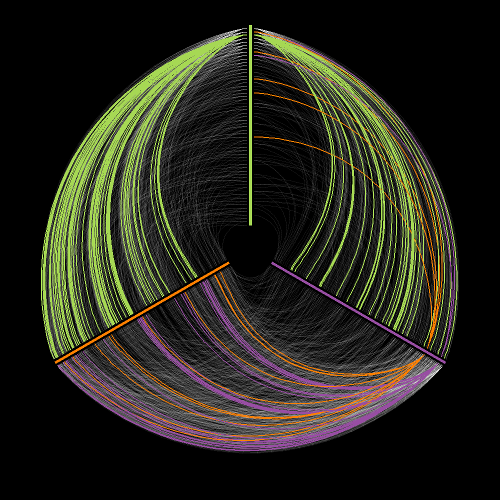
\includegraphics[scale=0.5]{hiveplotEx1}
	\caption{Example of a HivePlot containing 2500 vertices and 5900 edges.}
	\label{fig:hive_plot}
\end{figure}

Initially before the layout is made a number of structural parameters are calculated. Such as degree, flow, pagerank, clustering coefficient etc. Which parameters to use is up to the user to decide, they need to be appropriate for the network
being visualized. For example one could use the clustering coefficient to distinguish between hubs and clusters. Next these parameters are used to set up rules that are used to assign nodes to an axis and decide its coordinate. These rules
are often boolean rules. Example of rules could be: \
\begin{itemize}
	\item{Is the node a sink?}
	\item{Is the node a source?}
	\item{Clustering coefficient < 0.5?}
\end{itemize}
\

If a HivePlot can be created with three axes this is preferred \cite{Krzywinski01092012}, laying the axis with a uniform radial distribution. Because with three axis you get a layout that is edge crossing free. In addition to this 
three axis makes it possible for each edge between each axis pair not to cross another axis. Though this is not restrained to only three axis, it can be hard to partition nodes to axis so that nodes on axis are only connected
to neighbouring axis.

For hive plots there are some choices of use, one used is a Java based library \cite{website:JHive}. There are also libraries for R\cite{website:R}, HiveR\cite{website:HiveR}, that supports hive plots in the two-dimensional and three-dimensional space.
The framework D3.JS\cite{website:D3JS} is an other option that is a JavaScript to create hive plots. And pyveplot\cite{website:pyveplot} that is a library for hiveplots in Python\cite{website:python}.
\subsection{TreeMap}
TreeMap is a technique to present graphs in sequences of nested boxes \cite{herman00}. TreeMap requires the data to be hierarchy structured as a tree. Figure \ref{fig:tree_map_ex} shows an example. The size of individual boxes becomes significant in 
a TreeMap layout, where the user specifies how they should grow. Take for example if figure \ref{fig:tree_map_ex} shows data that represents a file system. The size of a box could then be proportional to the size of the file it represents. The colors of the boxes 
represent the hierarchy, same color of boxes belong to the same file.

For Treemaps there are some choices to use. For .Net, which is this thesis working environment, there is the WPF Treemaps \& SquarifiedTreeMaps control library\cite{website:WPFTreeMaps}, though it has poor documentation.
 Another alternative is the .NET Treemap Control library\cite{website:devxTreeMap}. Here again the problem lies in little documentation and it is hard to get information about the library when it was part of an old Microsoft
 research project called Netscan.
\begin{figure}[!htbp]
	\centering
	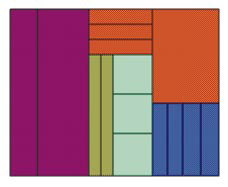
\includegraphics{TreeMapEx}
	\caption{Example of a Tree-map}
	\label{fig:tree_map_ex}
\end{figure}
\newpage
\section{Three-dimensional space}
In the hope of acquire more space for the layout of a network one can take the approach to go from a 2D to a 3D environment. In other words one can strive to get away from the euclidean space to another space that provides more space.
 An important aspect that follows going to a 3D view is that the system should be nagivatable. This because in a 3D view, node and edge occlusion is bound to happen. Being able to alter a view by navigating becomes an important tool 
 that helps to find a view where no occlusions occur.
\subsubsection{Hyperbolic space}
The hyperbolic space has the property that it has more room compared to the familiar euclidean space \cite{636718}. \cite{Wolfe} states that the fifth postulate in the Euclidean plane geometry can be formulated as: 
\begin{quote}
Through a given point, not on a given line, one and only one line can be drawn which does not intersect the given line.
\end{quote}
 As in the hyperbolic plane geometry they introduce the Characteristic Postulate:
\begin{quote}
Through a given point, not on a given line, more than one line can be drawn not intersecting the given line.
\end{quote}
Moreover two lines that are parallel in the euclidean space are always the same distance apart. As in the hyperbolic space parallel lines are not equidistant. For instance two parallel lines in the hyperbolic space that do 
not intersect can be seperated by increasing distance the further away one moves from the origin. Figure \ref{fig:hyperbolic_comp} shows this compared to the euclidean geometry.

\begin{figure}[!htbp]
	\centering
	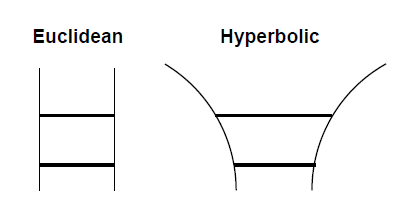
\includegraphics{HyperBolicGeom}
	\caption{Parallel lines in euclidean space are always the same
distance apart. In hyperbolic space the distance between
two lines that never meet does indeed change. Here we show two
geodesics which never meet but are not equidistant: the further they
extend away from the origin, the more room there is between them.}
	\label{fig:hyperbolic_comp}
\end{figure}

Normally to make use of the hyperbolic space, to use the extra space, one goes about to perform an layout algorithm in the hyperbolic plane or space and then display the results in the Euclidean plane or space. Some models
to do this have been created. Best known are the Klein and the Poincar\'e  models \cite{herman00}.
\subsection{GerbilSphere}
\label{Gerbil:chap2}
There have been studies on 2D vs 3D user interfaces that have shown that in many cases 2D exceeds 3D. Though the more space in 3D is still compelling. GerbilSphere is an inner sphere 2D system that tries to 
use the benefits from both a 2D approach as well as a 3D approach.

GerbilSphere works in a way that it place the observer inside a sphere while projecting the network on to the surface of the sphere. As part of the layout, GerbilSphere uses an extended version of the
 Fruchterman and Reingold force-directed algorithm to apply to the three dimensional space. However this is not enough to work on the surface of a sphere. To apply the forces to the surface of a sphere, GerbilSphere uses a 
 algorithm described by Kobeourov and Wampler \cite{kobourov}. For more technical information about the data structure and how their layout algorithm works see \cite{Shelley20121016}.

Zooming in GerbilSphere is viewed as having a world camera attached to one end of a tether and having the other end attached to the center of the sphere. When zooming in and out it can be seen as moving the world camera along this 
tether. Figure \ref{fig:gerbil_zoom} shows when zoomed out respectively zoomed in.
\begin{figure}[!htbp]
	\centering
	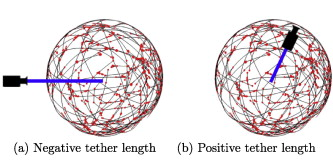
\includegraphics{GerbilZoomTether}
	\caption{Spherical volume grid based}
	\label{fig:gerbil_zoom}
\end{figure}

GerbilSphere implements a 2 1/2D interface, advocated by Ware\cite{Ware}. When a user is positioned inside the sphere and zoom in, the part of the network when zoomed in will be visualized on a flat 2D surface, as seen in Figure
\ref{fig:gerbil_POV}. When zooming out one can still have there point of interest in view, trying to gain more global context of the network. Lastly one can zoom
 out enough to place the view outside the sphere, seeing the network on a 3D sphere.
 
GerbilSphere is an open source project. No API is available, though good documentation is presented within the code.
 \begin{figure}[!htbp]
	\centering
	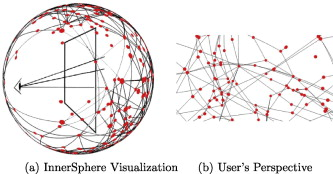
\includegraphics{GerbilPointOfView}
	\caption{Spherical volume grid based}
	\label{fig:gerbil_POV}
\end{figure}
\\
\subsection{H3: laying out large directed graphs in 3d hyperbolic space}
\cite{636718} visualize graphs in the three-dimensional hyperbolic space by placing the network, represented as a spanning trees, inside a sphere. Exploiting the property that the amount of space covered by a sphere
 in the three-dimensional hyperbolic space increases exponentially with respect to the radius of the sphere, rather than polynomially. They compare using the traditional cone trees with their use of a layout on spherical caps, 
 see figure \ref{fig:hyperbolic_cone_tree}.
 Figure \ref{fig:hyperbolic_example} shows an example of a network being displayed from \cite{636718}.
 
  \begin{figure}[!htbp]
	\centering
	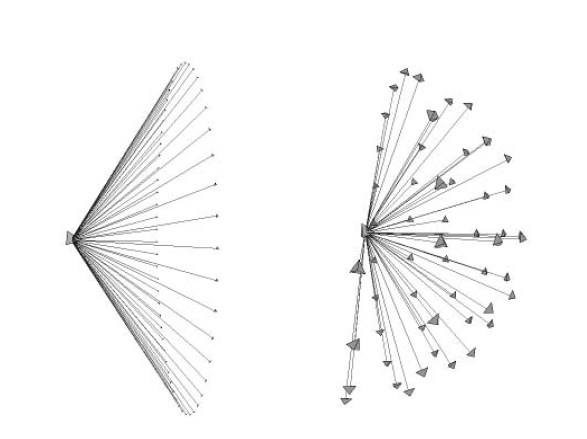
\includegraphics[scale=0.5]{H3ConeVSHem}
	\caption{Comparison of the traditional cone tree layout along the circumference
of a circle with the H3 layout on the surface of the spherical
cap. Both pictures show 54 child nodes in hyperbolic space, represented
by pyramids of the same size. Left: The traditional perimeter
layout requires a large cone radius and is quite sparse. Right: A
quite small cone radius suffices for the H3 spherical cap, so the layout
is reasonably dense.}
	\label{fig:hyperbolic_cone_tree}
\end{figure}
 
 \begin{figure}[!htbp]
	\centering
	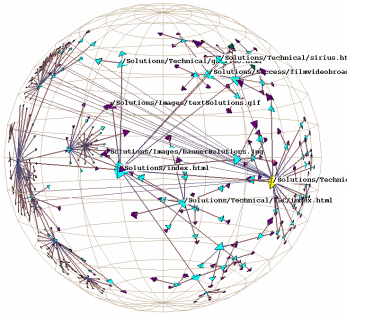
\includegraphics[scale=0.5]{HyperBolicEx1}
	\caption{Link structure of a Web site laid out in Three-dimensional hyperbolic space by \cite{636718}. The nodes represent documents,which are coloured
according to MIME type: HTML is cyan, images are purple, and so on.}
	\label{fig:hyperbolic_example}
\end{figure}

\newpage
\section{Looking forward}
After the information that has been undergone in this chapter how do we procede in the future chapters of this thesis? 
When this thesis has been done within a time constraint all relative methods of visualisation could not be implemented and evaluated due to the great number of existing methods. Still measures need to be
taken so that no major or relevant visualisation method gets overlooked. With the information presented in this chapter as a basis, the visualisation techniques of the highest relevance will be
 chosen for evaluation.
\subsubsection{Space}
One important choice of consideration is in which space should the networks be displayed? In this chapter the reader were introduced to a number of different spaces where also different
 visualisation methods have been evaluated with specific data as described. One can conclude that the two most common spaces, the two- and three-dimensional space, are of great importance and need
 to be included for this thesis purpose.

Different visualisation techniques will behave differently and result in having different aspects and characteristics depending on which space one uses. These can then be compared for evaluation purposes,
such as how layout of nodes and edges differs and what impact the space has on zooming and panning. Also how label clutter behave in different spaces may be of interest.

\subsubsection{Layout method}
When it comes to choosing which layout methods to evaluate, the same aspects mentioned in the previous section needs to be considered here as well. Which layout method one chooses to use can have a hugh 
impact on these aspects. Their results may also differ depending on which space one use and it needs to be taken into consideration.
 
\subsubsection{Chosen views}
\label{chosen-views}
From the research and study in this chapter a selection narrowed down to three different views where made to be used for a implementation of an application. In this selection both the two-dimensional and the 
three-dimensional space were covered. We will show the resulting application and for each view give an account of why that view where selected and how it was implemented in \ref{sec:application}.

\subsubsection{Technical aspects}
In addition to the effects on visualisation from different selection on spaces and layout methods there are other more practical aspects to be considered. Aspects revolving around one enforcing some pretension
 on the performance of the chosen methods implemented. This to ensure smooth usage so that a slow visualisation application will not impact the result in a negative way when evaluating a visualisation technique.
 More about this in section in the next chapter and appendix \ref{app:library:evaluation}.
 
\chapter{Method}
\label{chap:three}
When one is to display data using graphs one is confronted with the task of choosing between a large range of different visualisation techniques.
This chapter is intended to show the prosess used to decide which methods and areas to be investigated for this thesis. In section \ref{sec:Implementation} 
the way found to implement these choices for further evaluation is shown. In section \ref{sec:evaluation} the way taken for evaluation is described.
\section{Implementation}
\label{sec:Implementation} 
It is difficult to compare and evaluate different visualisation techniques only on the information found in scientific thesis and books concerning them. 
One cause to this arises when one looks at the data used, different theses use different data. In some cases data might seem bias, having been chosen to fit better with the 
visualisation method concerned for the purpose of that particular thesis, making it hard to compare performance between techniques. Different visualisation methods perform differently on different data, making it 
only helpful if one wants to establish some form of knowledge around that a specific technique can be good on a specific kind of data. For this thesis it was necessary to have a more generalized unbiased approach.

To work around this an implementation were to be made that incorporates a selection of the studied techniques. Following the methodologies of selection for spaces and layout methods discussed earlier.
This in order to make it possible to display the same networks (same data), using these different techniques and then be able to compare and evaluate performance on these techniques.
\subsection{Programming environment}
The implementation was to be developed in the programming language C\# \space (C-sharp)\cite{website:MSDN} within Visual Studio\cite{website:VisualStudio}. 
The main application was to be made as an WPF (Windows Presentation Foundation)\cite{website:WPF}. Other programming languages that have been used and incorporated in to the main WPF application is C++\cite{website:C++} 
and Java\cite{website:Java}. For database retrieval LINQ (Language-Integrated Query)\cite{website:LINQ} has been used.
\section{Evaluation}
\label{sec:evaluation}
In order to draw some relevant results from this thesis it is necessary to evaluate the different visualisation techniques chosen to be investigated. Section \ref{sec:evaluation:layoutviews} will  
explain different aspects that needs to be considered when evaluating the different layout methods. Section \ref{sec:evaluation:libraries} takes up the necessity to adding tests concerning not
 only layout methods but also on the prerequisites for implementing these, which programming libraries to use.
\subsection{Layout views}
\label{sec:evaluation:layoutviews}
Based on the study done in chapter \ref{Theory} the different views will be evaluated on the following characteristics that are of great importance for a general visualisation system:\
\begin{itemize}
	\item{Navigation}
	\item{Situational awareness}
	\item{Ease of recognizing important parts as sub-networks, nodes and connections}
	\item{Labelling}
\end{itemize}
\
The evaluation will be executed by using the implemented application to try and complete tasks similar to the following:\
\begin{itemize}
	\item{Identify cluster/node X. Navigate to cluster/node Y. Can one navigate back to X?}
	\item{Identify the biggest cluster}
	\item{Identify node X}
	\item{Identify the node with highest degree}
\end{itemize}
\
The tasks will be viewed as completed correctly, incorrectly or uncompleted. In addition to this, time will be taken into consideration as a measurement of performance. The results and drawn conclusions from these evaluations
can be found in chapter \ref{chapter:five}.
\subsection{Programming libraries}
\label{sec:evaluation:libraries}
An evaluation of different programming libraries was made to find a good starting point for the implementation of an application. First a study that investigates what different libraries exists that supports visualisation 
for different networks was made. In this research a comparison of which different functionality these libraries supports were retrieved in form of data structures and algorithms, layout algorithms and so on.

From this first initial study a selection of possible libraries to use for implementation were needed to be made. From here one could then evaluate the different selections to be able to make a final choice
 of which libraries to use.

The library evaluation will test for the libraries capacity in speed, how long time does it take to set up and draw networks of different sizes? And then as the last step was to evaluate the performance 
of the libraries after the networks had been drawn. This by taking measurements of smoothness while traversing a network. Were smoothness was represented by the applications FPS while navigating the 
network at different stages. The evaluation of programming libraries can be found in appendix \ref{app:library:evaluation}.
\subsection{Data}
To be able to perform these evaluations some data needs to be at hand, data that fits this thesis purpose. This thesis has been performed at a company that provided the necessary data to be visualized.
\subsection{Data for layout views}
\label{data:layout-views}
For the layout views, data in the form of electronical units found inside trucks called ECUs (Electronic Control Units) are used. Also variables used within these systems called AEs (allocation elements)
 are used to be visualized. 
 
This data have a complex form with a great number of relations and communications, not suiting some visualisation techniques more then others, thus making it suitable as data for this thesis purpose.
\subsection{Data for evaluation of programming libraries}
For the performance evaluation of programming libraries data were needed to be generated. To generate this data the program Gephi\cite{website:gephi} was used. This program was to be used to generate a number of different 
graphs of different sizes which was then saved as a plain text file. The following graphs were generated:\
\begin{itemize}
	\item{Graph with 50 vertices with 592 edges. Referred as G50.}
	\item{Graph with 100 vertices with 3941 edges. Referred as G100.}
	\item{Graph with 500 vertices with 99641 edges. Referred as G500.}
	\item{Graph with 1000 vertices with 399969 edges. Referred as G1000.}
\end{itemize}

On the account that different libraries use different ways of representing data this text file can not be presumed to work as input for all libraries. On that fact parsers were needed to be developed to
attend that the input was on the right format for the corresponding library.
\chapter{Results}
\label{chap:results}
This chapter narrate the results produced from the literature studies and the application that was implemented. The results from an evaluation of excisting programming
libraires are given in section \ref{sec:libperform}. For a more ingoing review of these libraries and how they were evaluated see appendix \ref{app:library:evaluation}. 
Section \ref{sec:application} shows the resulting application from the implementation and its views.  
\section{Library performance}
\label{sec:libperform}
To be able to make a solid application that can be used for this thesis evaluations, not only the need (though it is most of importance) of choosing what layout methods to be used needs to be considered. Under which prerequisites
one chooses to use while implementing said application needs to be considered. Thereby a consideration of which libraries one can use when implementing the different visualisation methods is needed.
\subsection{Attribute matrix}
\label{Lib:attribute}
\newline
\\
The following matrix, Figure \ref{fig:AttributeMatrix}, lists important functionality one looks for when considering a programming library for implementing visualisation methods. The matrix gives an overview of what the 
different libraries supports from the start. This matrix helps as a basis when selecting libraries for the implementation.\\

\begin{figure}[!htbp]
	\centering
	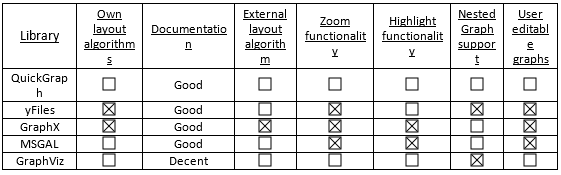
\includegraphics[scale=1.0]{LibraryAttributeMatrix}
	\caption{Attribute matrix}
	\label{fig:AttributeMatrix}
\end{figure}

\newpage
\subsection{Results from library tests}
\label{sec:lib:results}
\textbf{\textit{Speed}}\\
\newline
Each graph have been drawn ten times and the arithmetic mean value of the time has been calculated and given as result. Time is displayed on the form of minutes:seconds.\

\newline
\begin{table}[h]
\centering
\caption{Speed results}
\begin{tabular}{|c|l|l|l|l|}
\hline
\multicolumn{1}{|l|}{} & \multicolumn{1}{c|}{\textbf{G50}} & \multicolumn{1}{c|}{\textbf{G100}} & \multicolumn{1}{c|}{\textbf{G500}} & \multicolumn{1}{c|}{\textbf{G1000}} \\ \hline
\textbf{GraphX}        & 00:00.51461281                    & 00:07.41482771                     & 22:33.4573175                      & Out of memory                       \\ \hline
\textbf{VTK}           & 00:00.01546258                    & 00:00.04138581                     & 00:00.88301525                     & 00:03.53977976                      \\ \hline
\textbf{yFiles}        & 00:00.54974544                    & 00:01.68249026                     & 00:49.60542746                     & 12:11.535764772                     \\ \hline
\end{tabular}
\label{table:librarie-speed}
\end{table}
\newline
\textbf{\textit{Smoothness - FPS(Frames per second)}}\\
\newline
There are three fps measurements for each library were panning actions was being performed. One zoomed out far away, giving an overview of the
graph (Z1), one zoomed in half way to the centre of the graph (Z2) and a third were the user are zoomed far in to the graph, being able to distinguish between vertices (Z3).
\newpage
\begin{table}[h]
\centering
\caption{GraphX}
\begin{tabular}{|c|c|c|c|}
\hline
\multicolumn{1}{|l|}{} & \textbf{Z1}    & \textbf{Z2}    & \textbf{Z3}    \\ \hline
\textbf{G50}           & 17 fps         & 23 fps         & 35 fps         \\ \hline
\textbf{G100}          & 1 fps          & 3 fps          & 5 fps          \\ \hline
\textbf{G500}          & Undetectable   & Undetectable   & Undetectable   \\ \hline
\textbf{G1000}         & Non-executable & Non-executable & Non-executable \\ \hline
\end{tabular}
\label{table-graphx}
\end{table}
\newline
\begin{table}[h]
\centering
\caption{VTK}
\begin{tabular}{|c|c|c|c|}
\hline
\textbf{}      & \textbf{Z1} & \textbf{Z2} & \textbf{Z3} \\ \hline
\textbf{G50}   & 1000 fps    & 1000 fps    & 1000 fps    \\ \hline
\textbf{G100}  & 500 fps     & 500 fps     & 500 fps     \\ \hline
\textbf{G500}  & 35 fps      & 11 fps      & 3 fps       \\ \hline
\textbf{G1000} & 11 fps      & 7 fps       & 2 fps       \\ \hline
\end{tabular}
\label{table-VTK}
\end{table}
\newline
\begin{table}[h]
\centering
\caption{yFiles}
\begin{tabular}{|c|c|c|c|}
\hline
\textbf{}      & \textbf{Z1}  & \textbf{Z2}  & \textbf{Z3}  \\ \hline
\textbf{G50}   & 22 fps       & 20 fps       & 25 fps       \\ \hline
\textbf{G100}  & 2 fps        & 3 fps        & 5 fps        \\ \hline
\textbf{G500}  & Undetectable & Undetectable & Undetectable \\ \hline
\textbf{G1000} & Undetectable & Undetectable & 2 fps        \\ \hline
\end{tabular}
\label{table-yFiles}
\end{table}

\section{Application}
\label{sec:application}
This section shows the resulting application implemented with the corresponding views chosen from the research done in chapter \ref{Theory}.
\subsection{Main application}
At the start up of this application the user will be taken to the main application where the user will be prompted to make some choices before being able to visualize data. 
These choices are concerning which data to be used. 

In this application the user are constrained to choose between visualising ECUs or AEs, see section \ref{data:layout-views}. The user is also prompted to choose which SOP date to use. Next the user 
need to load the data from the database by pressing a button, labeled "Load Data". After that is done the user can then go on and choose which view to display. The user is not restrained to one view at the 
time but can bring up multiple views at the same time, making it easy to compare views.
\subsection{Force-Directed(FD) based view}
\label{FD-based-view}
Force-directed algorithms is, as shown in chapter \ref{Theory}, an important part when it comes to viualiseing networks. There are many visualisation techniques based solely on force-directed algorithms.
While other visualisation techniques that uses different approaches often incorporate some kind of force-directed algorithm to their visualisation method. As for example by computing a base graph using a
 force-directed algorithm. Therefore the first view of the implementation is a view that uses a force-directed algorithm for the vertices layout and edge routing. Figures \ref{fig:AllaAE2} to \ref{fig:AllaAesTwoDUnLabeled}
 show examples of the application using this view.

\begin{figure}[!htbp]
	\centering
	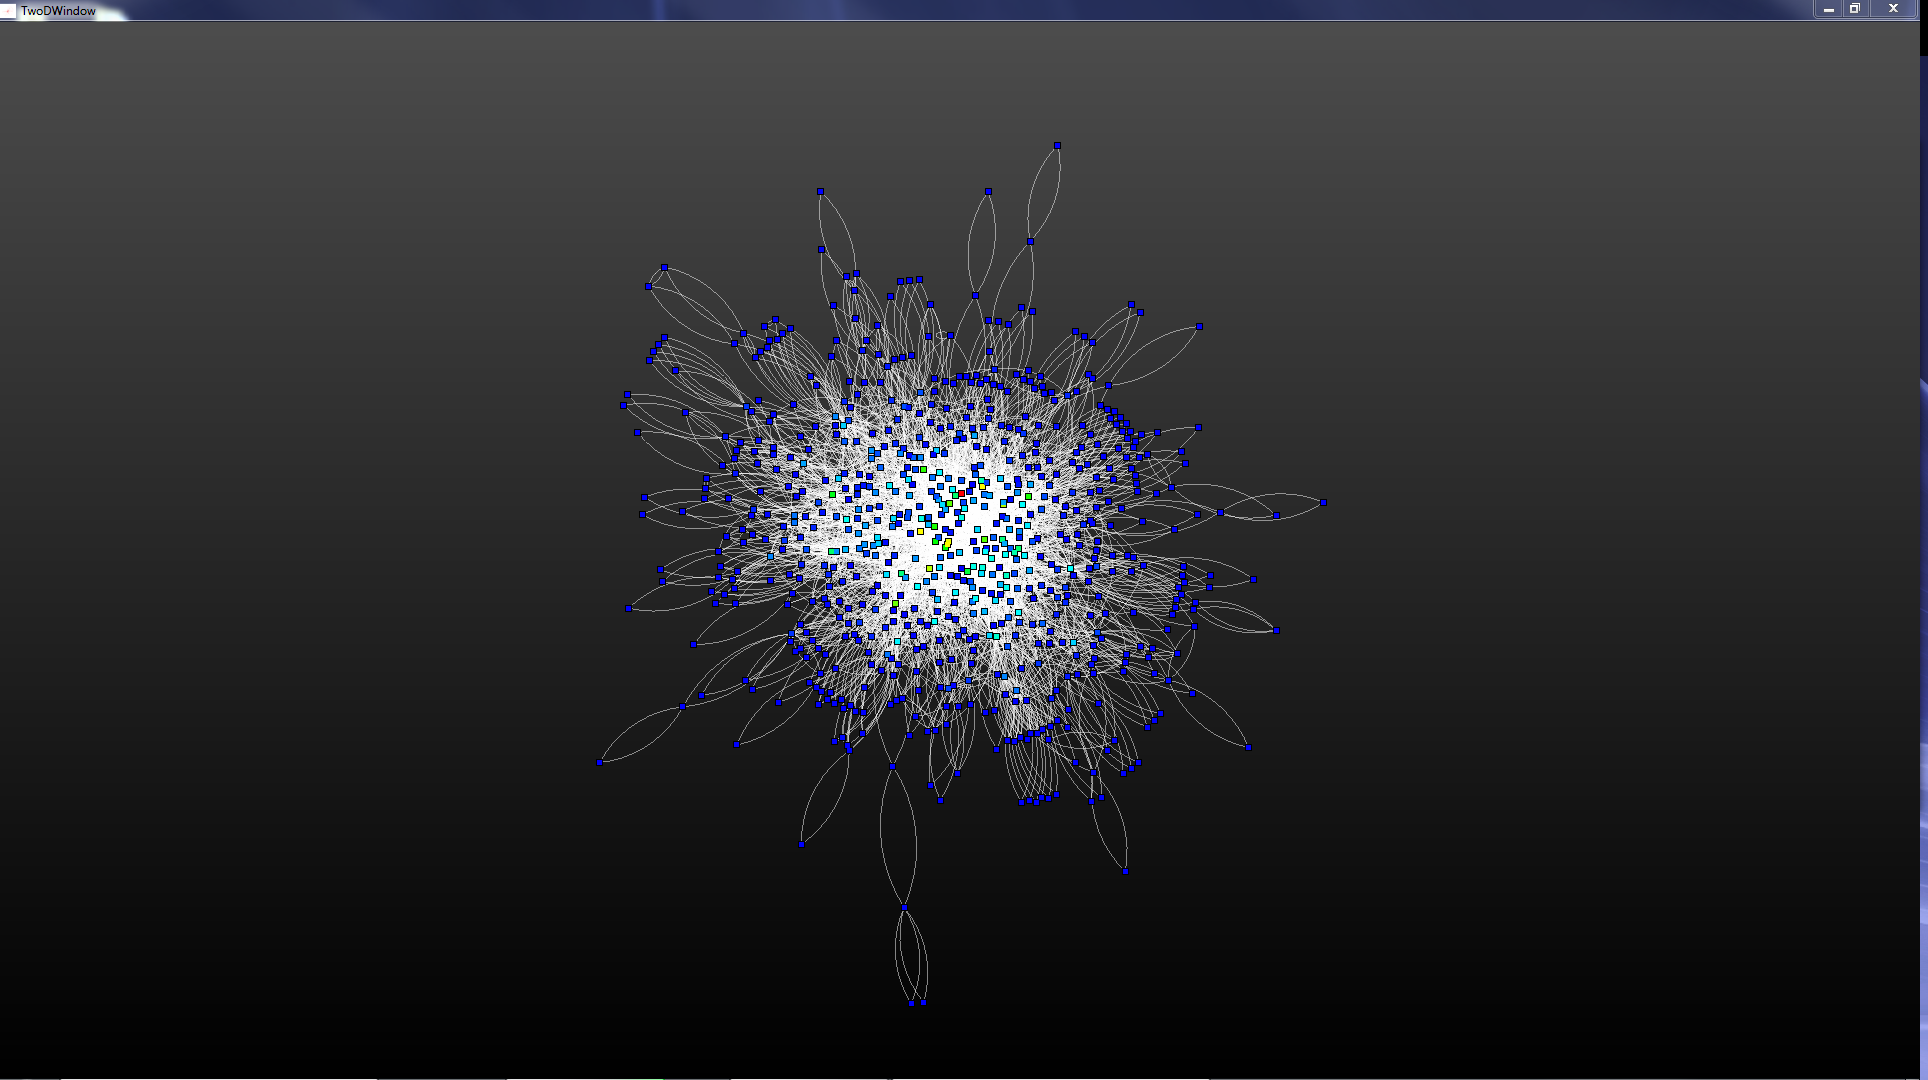
\includegraphics[scale=0.3]{SesammVisualAppPics/2D-View/Unlabled/AE/AllaAE2}
	\caption{An unlabled overview of a network were all AE was chosen.}
	\label{fig:AllaAE2}
\end{figure}

\newpage
\begin{figure}[!htbp]
	\centering
	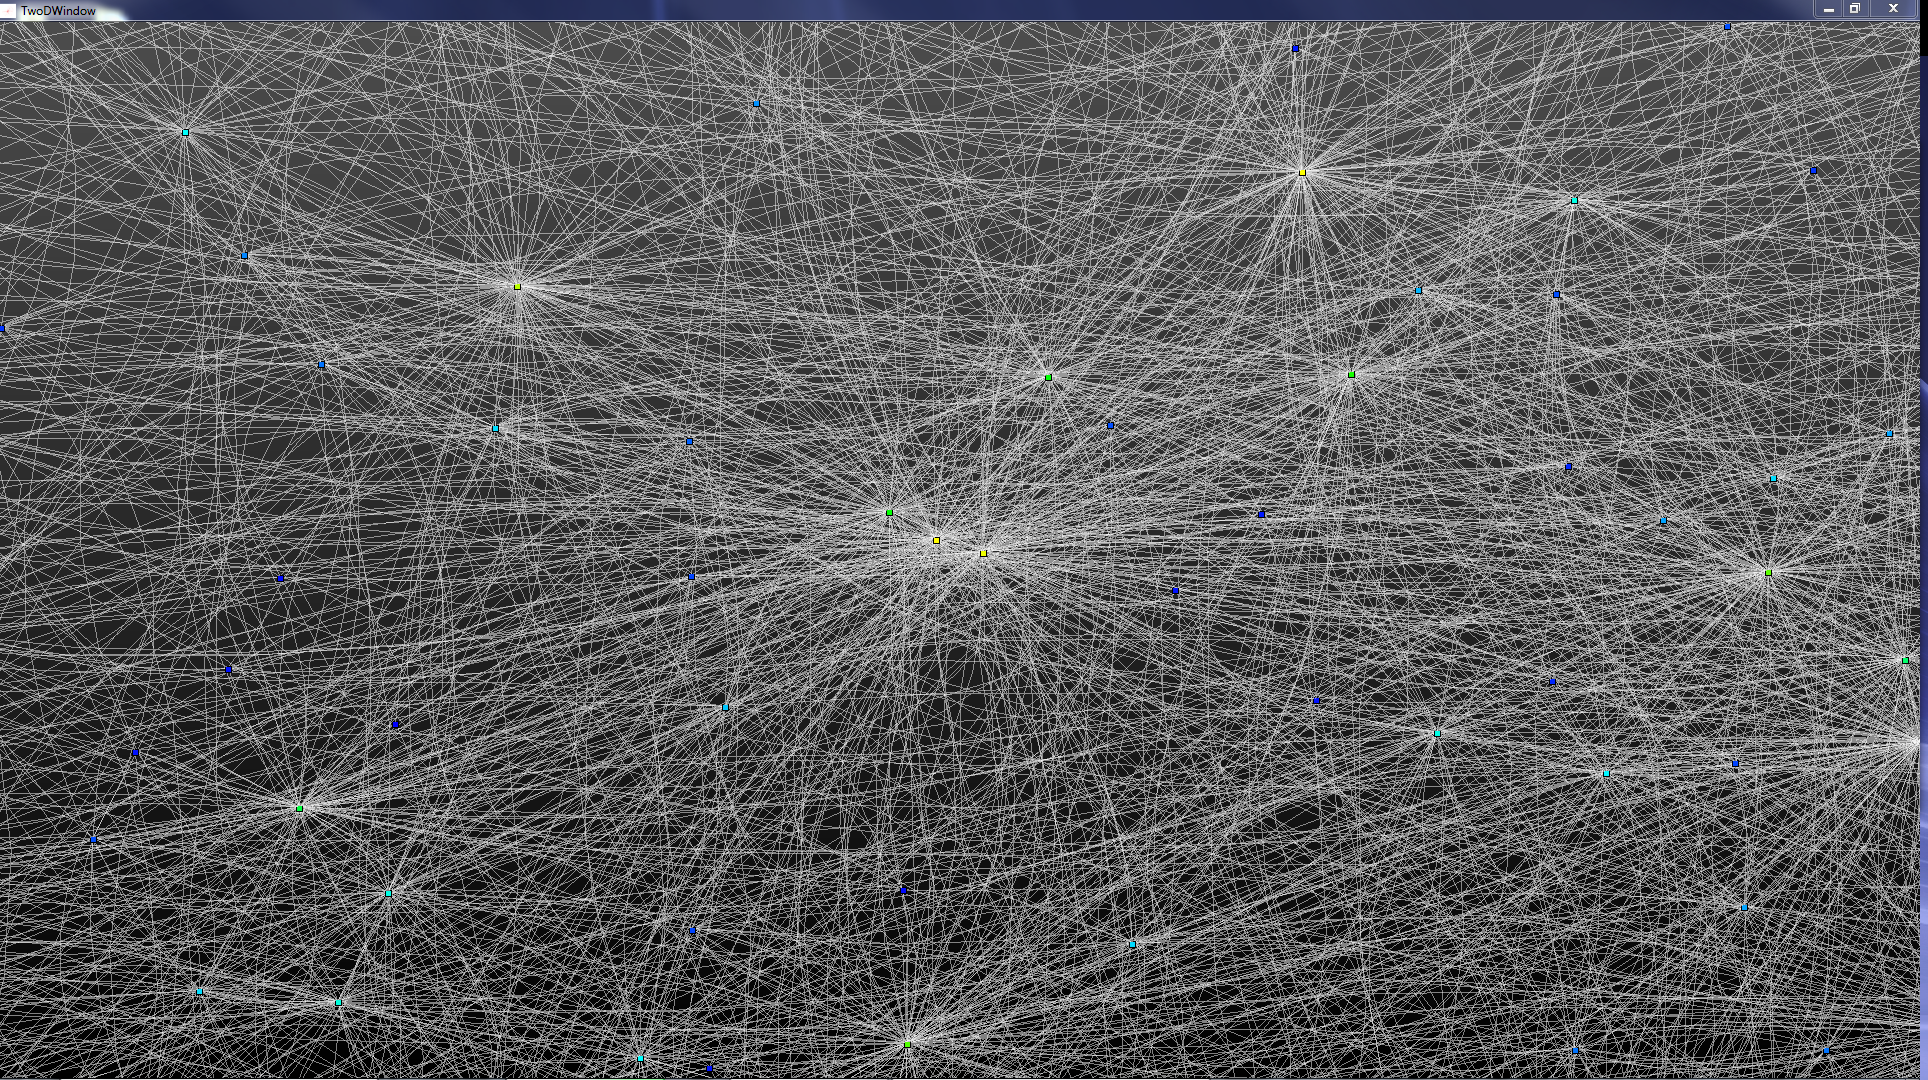
\includegraphics[scale=0.3]{SesammVisualAppPics/2D-View/Unlabled/AE/AllaAE4}
	\caption{Same network as in \ref{fig:AllaAE2} after zooming actions were preformed.}
	\label{fig:AllaAE4}
\end{figure}

\begin{figure}[!htbp]
	\centering
	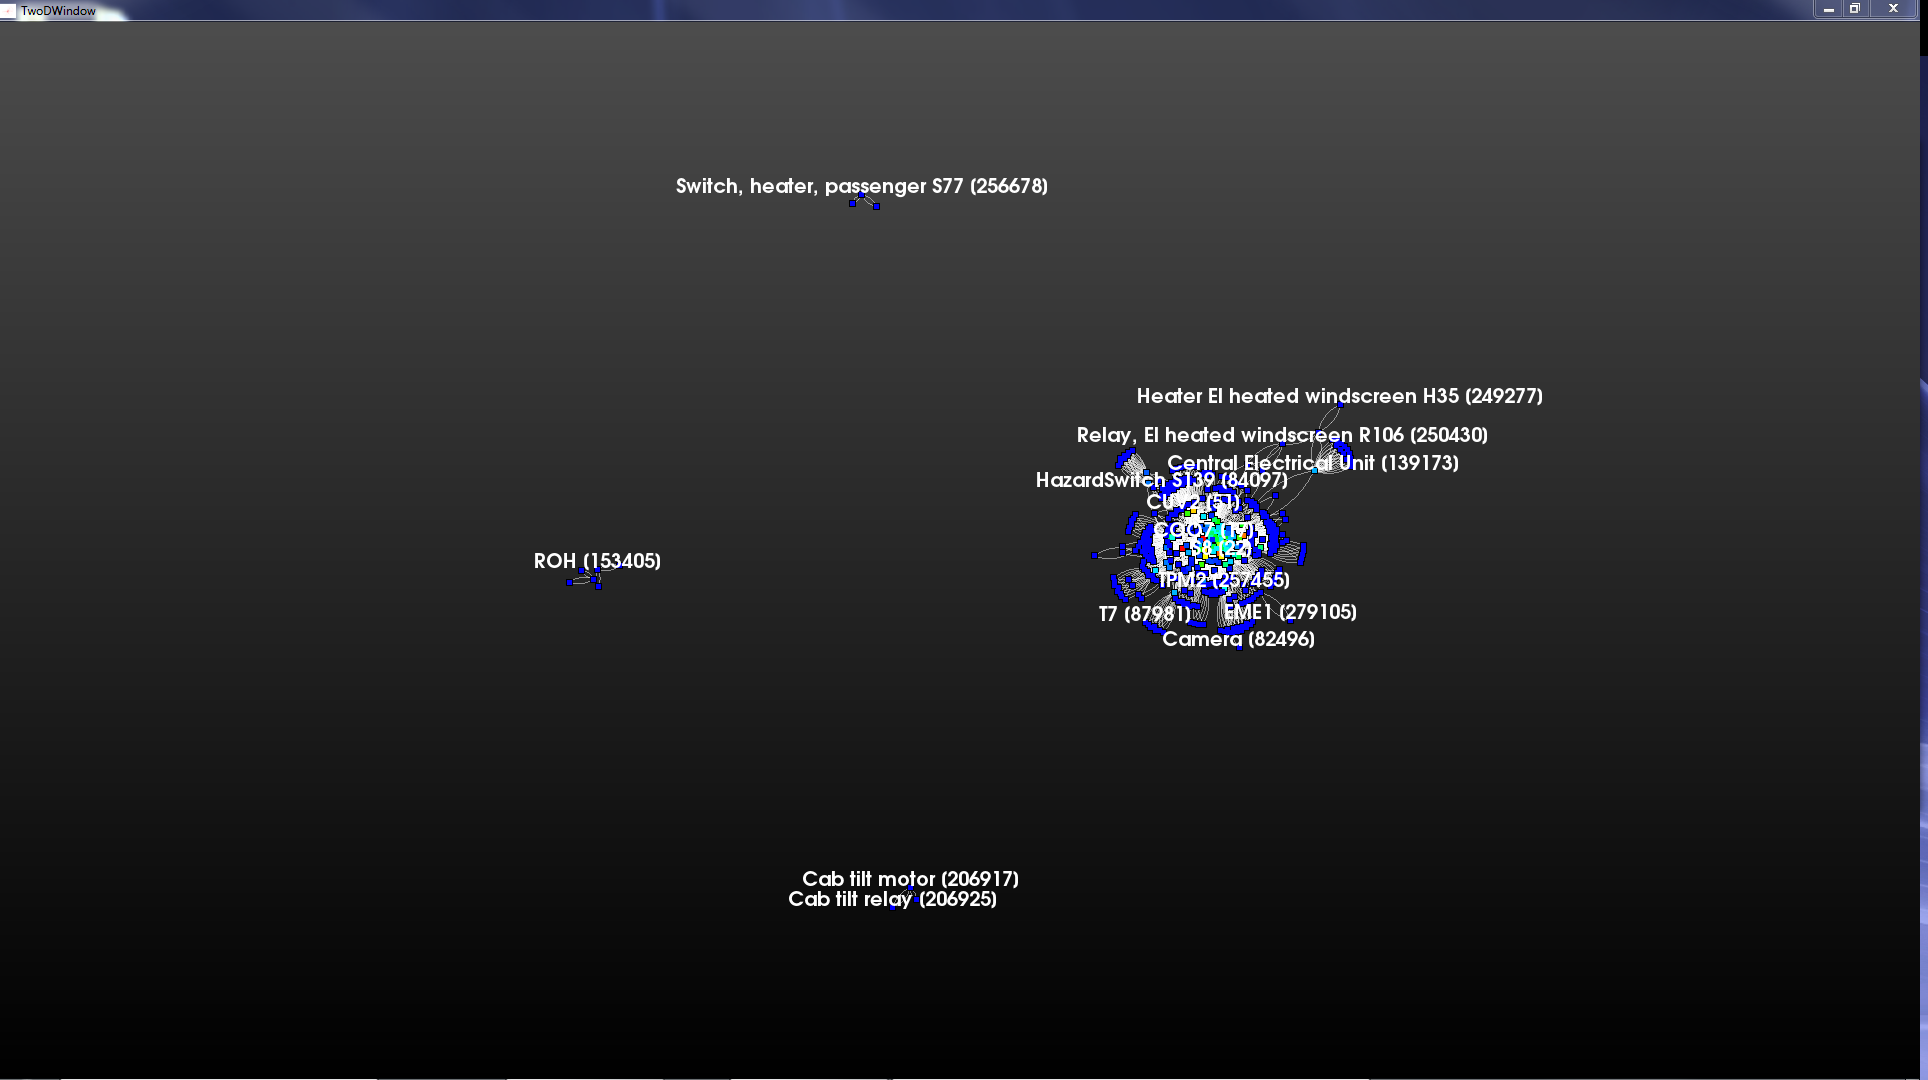
\includegraphics[scale=0.3]{SesammVisualAppPics/2D-View/Labled/ECU/AllaECU1}
	\caption{A labled overview of a network were all ECUs was chosen.}
	\label{fig:AllaECU1TwoD}
\end{figure}

\begin{figure}[!htbp]
	\centering
	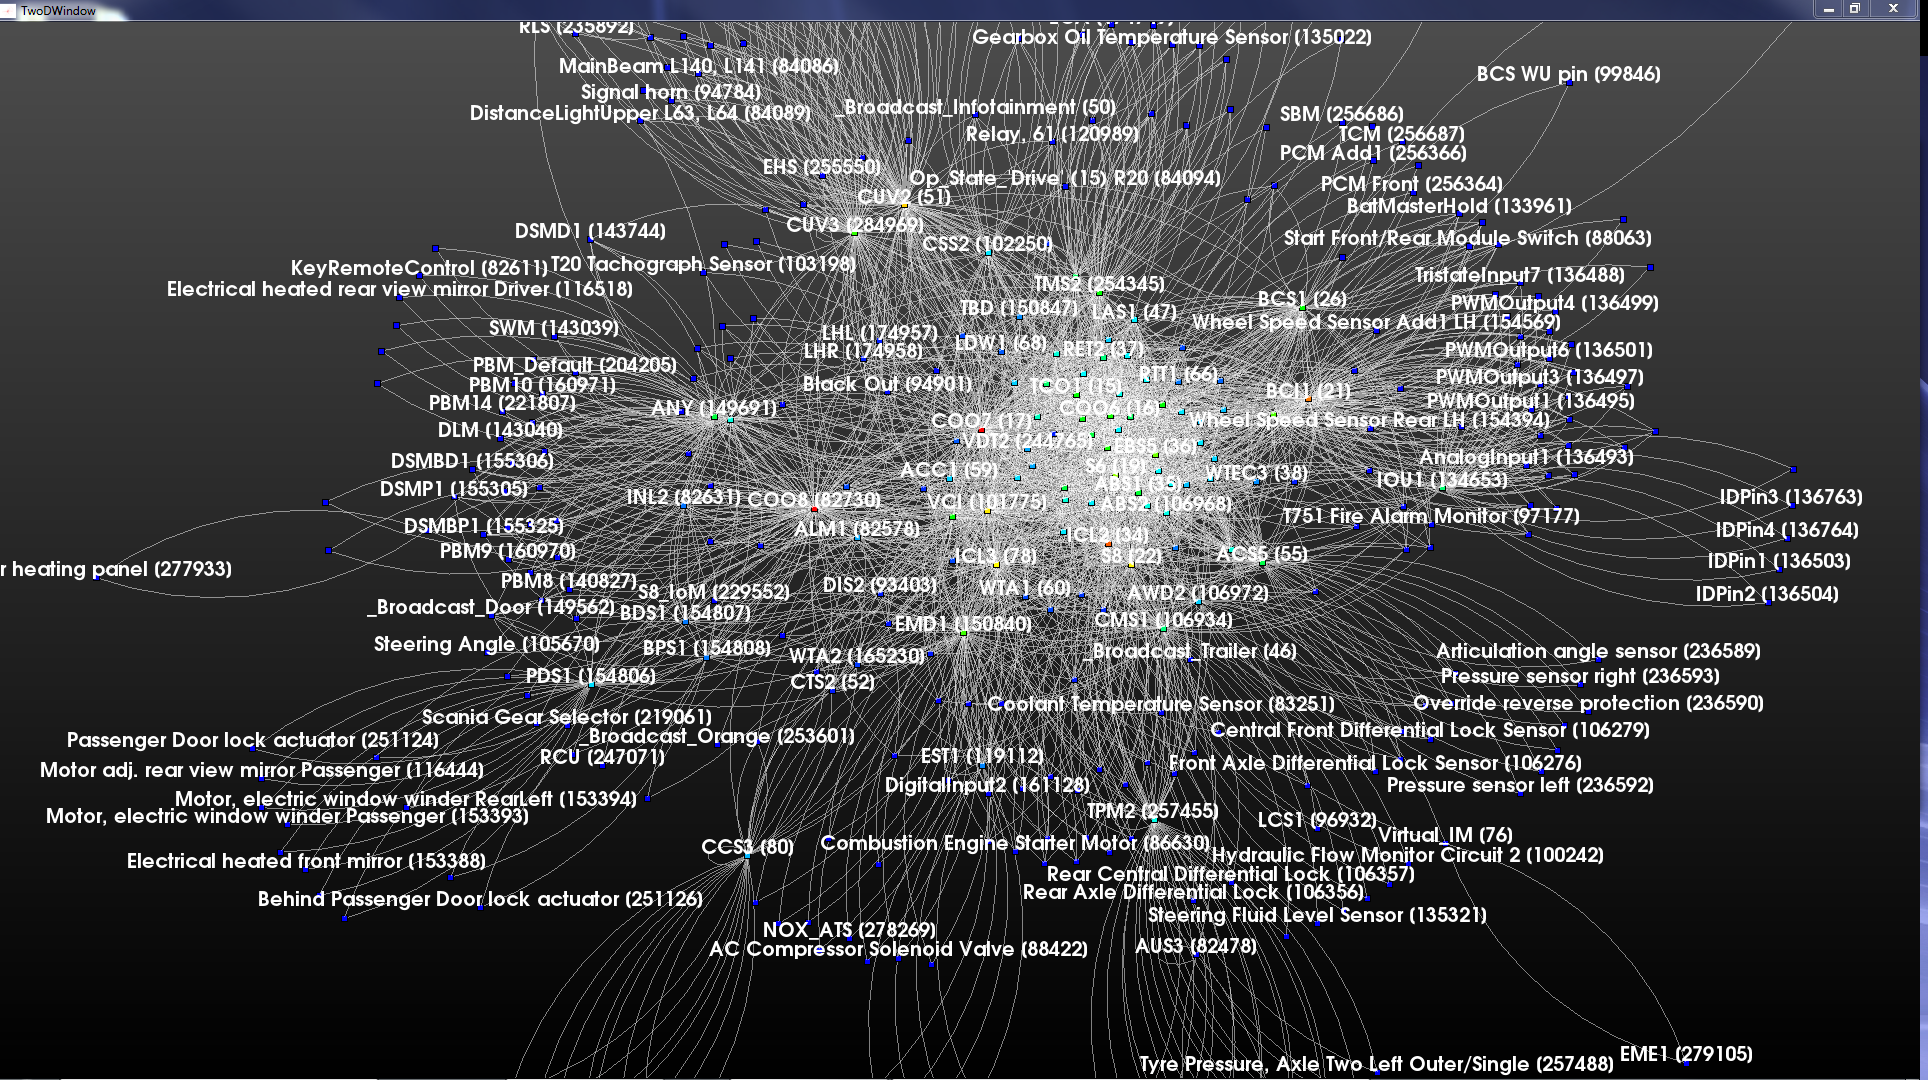
\includegraphics[scale=0.3]{SesammVisualAppPics/2D-View/Labled/ECU/AllaECU3}
	\caption{Same network as in \ref{fig:AllaECU1TwoD} after zooming actions where preformed.}
	\label{fig:AllaECU3TwoD}
\end{figure}

\newpage
 \begin{figure}[!htbp]
	\centering
	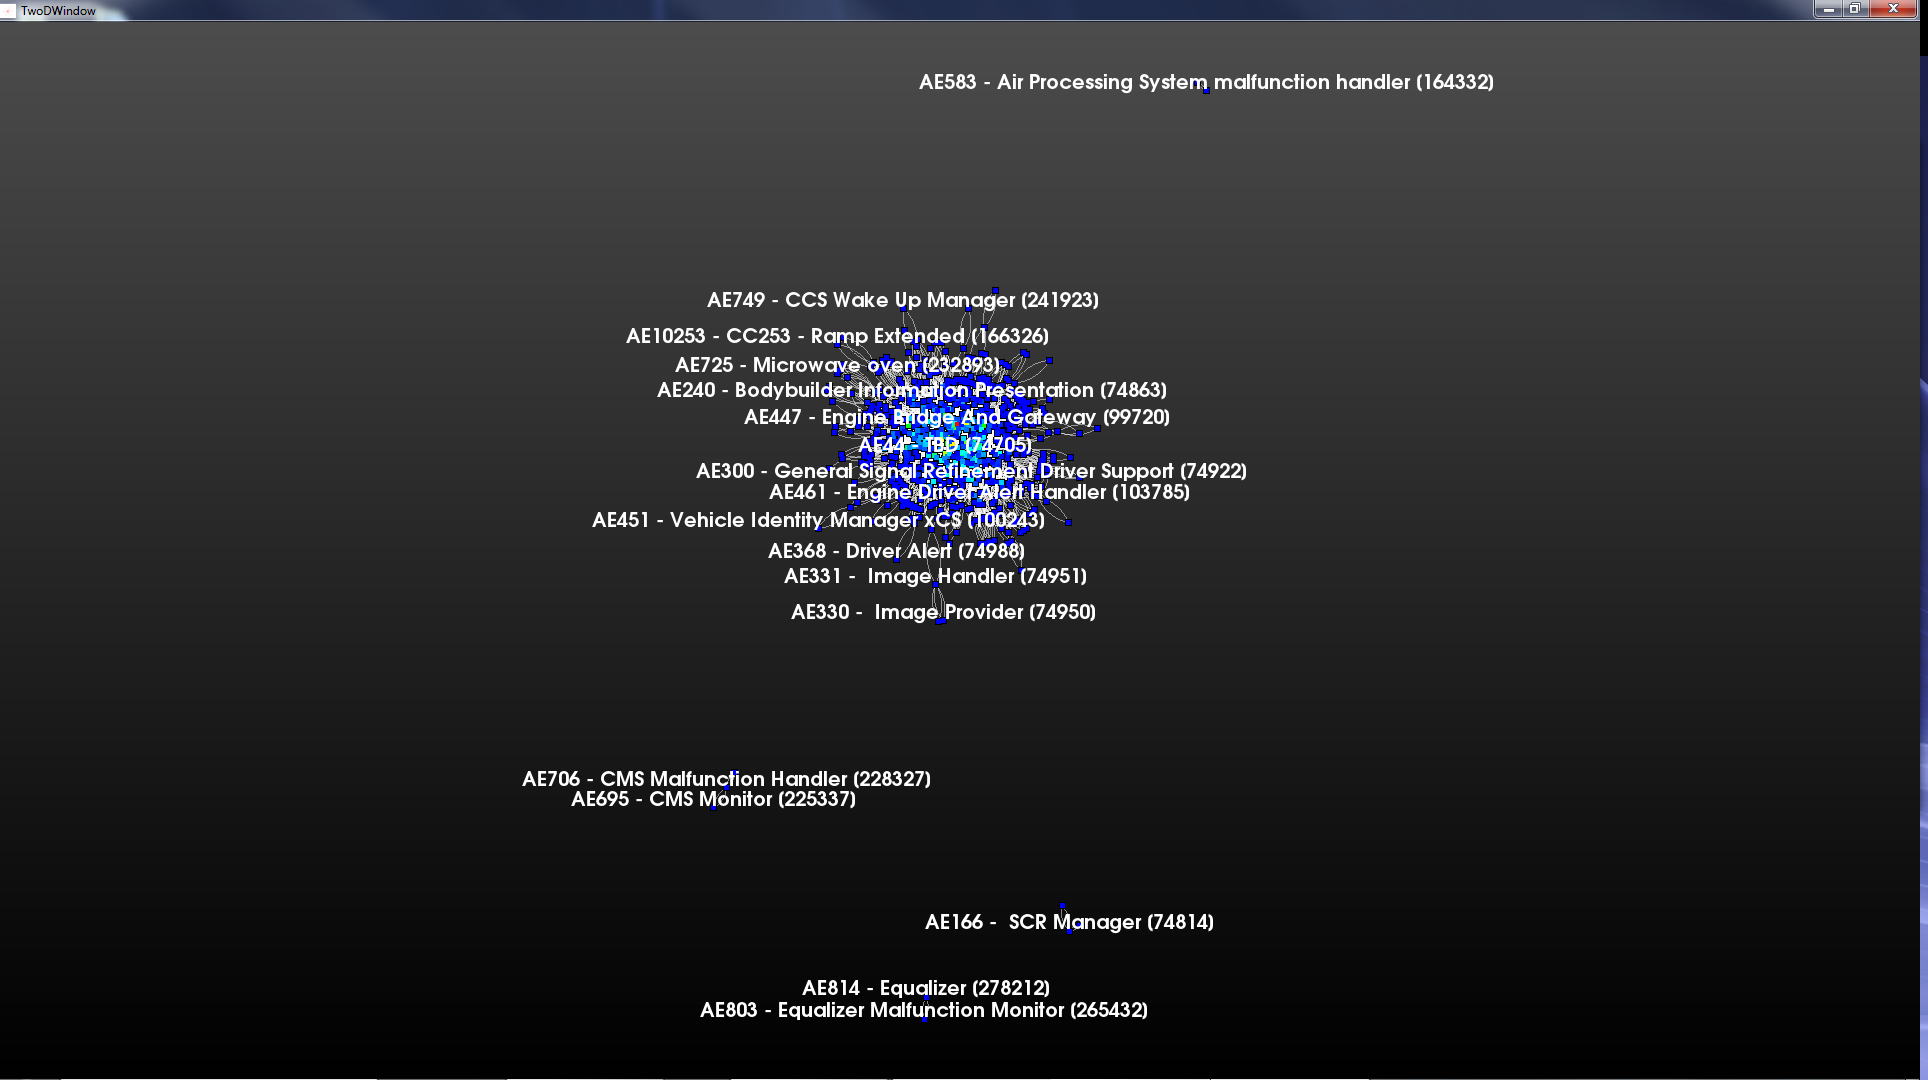
\includegraphics[scale=0.3]{SesammVisualAppPics/2D-View/Labled/AE/2D-View1}
	\caption{Showing data with labels enabled.}
	\label{fig:AllaAesTwoDLabeled}
\end{figure}

\begin{figure}[!htbp]
	\centering
	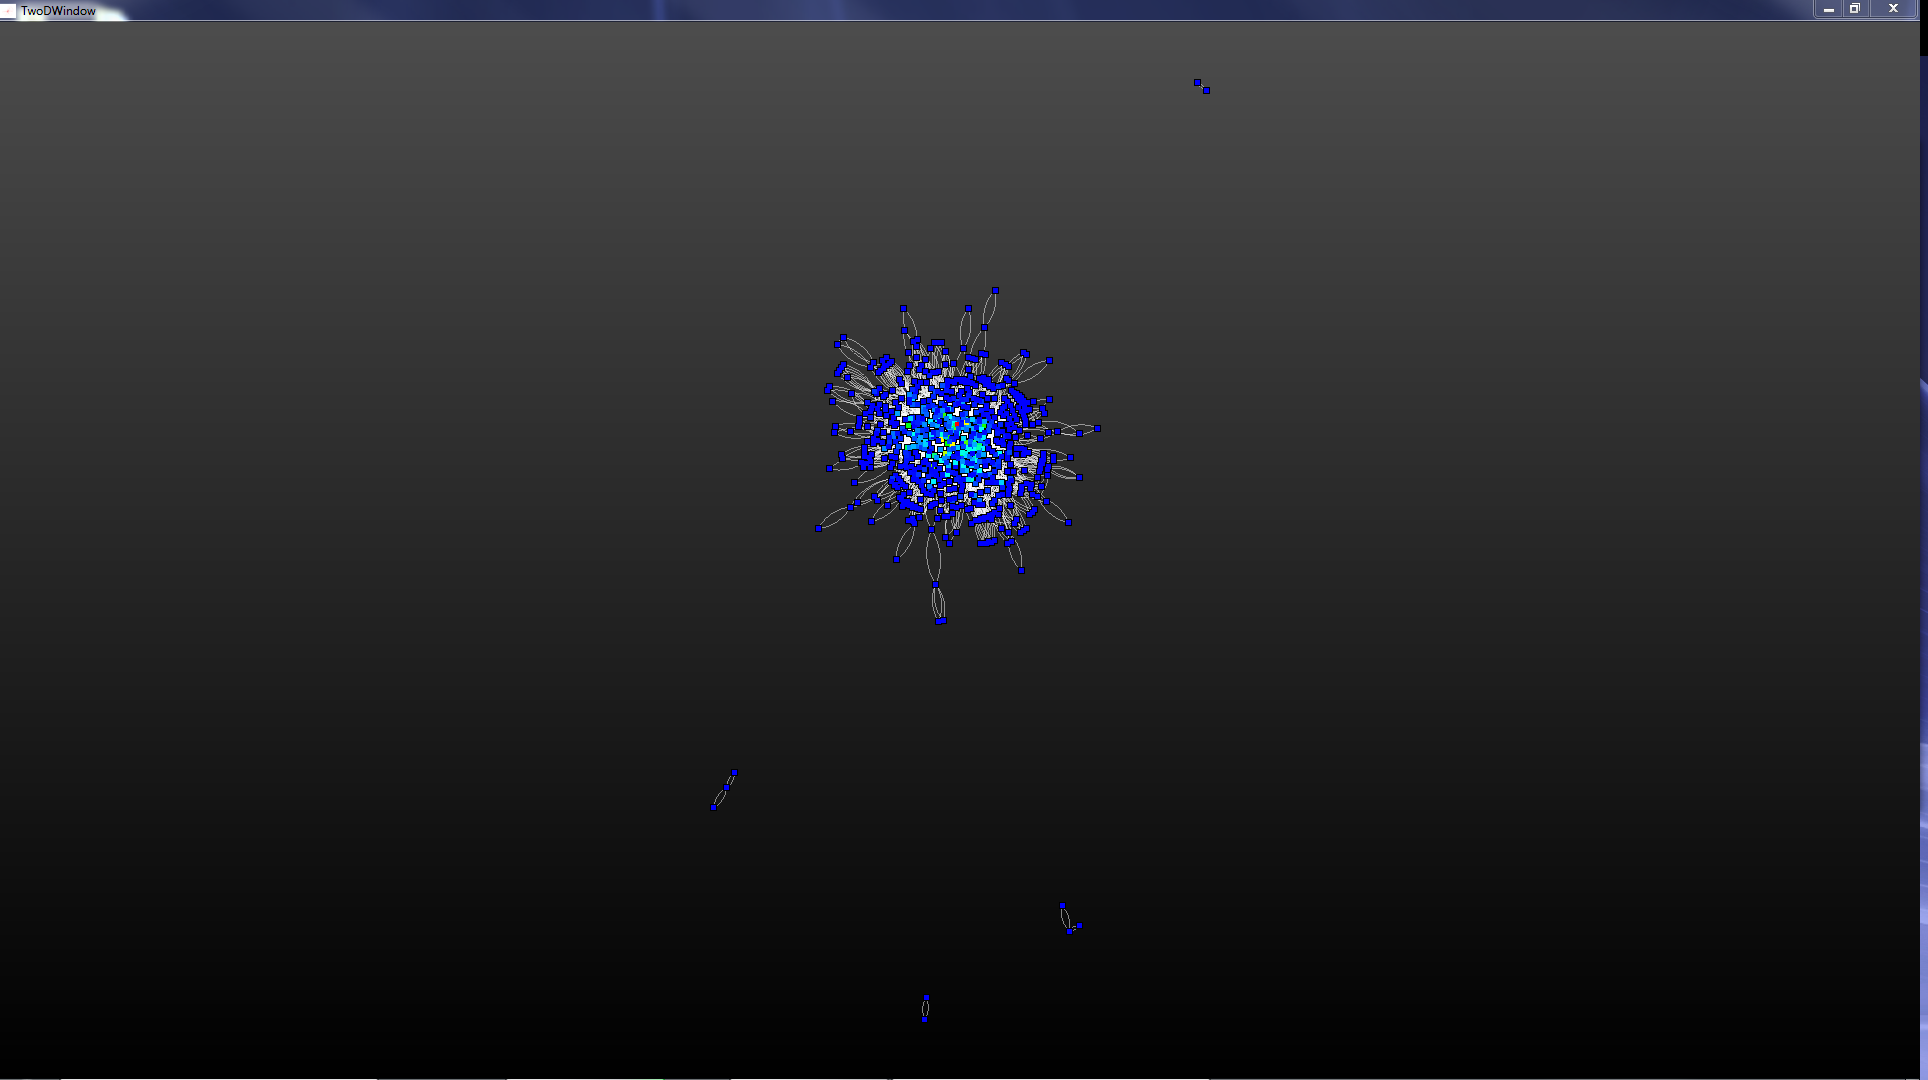
\includegraphics[scale=0.3]{SesammVisualAppPics/2D-View/Unlabled/AE/AllaAE1}
	\caption{Showing same data as in picture \ref{fig:AllaAesTwoDLabeled} but with lables unenabled.}
	\label{fig:AllaAesTwoDUnLabeled}
\end{figure}

\subsubsection{Labeling}
As mentioned in section \ref{FD:View:appendix}, the VTK library displays labels according to their weights, the higher the weight the higher priority a given vertice label will have. This combined with the force-directed algorithm by nature is good at evenly spreading out vertices, label 
obscuration becomes lesser of a problem. An example of this is shown in figure \ref{fig:AllaECU3TwoD} where a fairly large network is being displayed. 

Of course this comes at a price. By allowing a prioritizing of which labels to display one is left with a
loss of information, in this case a loss of labels. This can have a large effect on the outcome result when using
this application. Depending on what tasks one wants to solve by using this visualization technique, important
data may be missed and/or be more difficult to locate. It comes down to what data one is attempting to extract
from the view. If for instance one is out to identify the vertices with a large number of connections and greater subnets
this view might work terrific. On the other hand if one is to find a specific data part that may be smaller weighted this view can be difficult and uneasy to use.
\subsubsection{Navigation - Situational awareness}
The effect on the situational awareness of a user in this view depends highly on what stage in a task the user is on and what type of task said user is performing. Because the view
provides a highly zoomable network a user can with a far out zoomed view, combined with the labeling enabled, acquire a good overlook of a given network.

Though when zooming in using this view there comes a point when some data are lost, there
is only so much data that can fit on a screen at the same time. This can diminish the situational awareness for a user and result in
a loss of orientation, forcing a user to zoom out to try and see correlations from one part of the network to another. The user might even have a loss in orientation trying to get back to the same spot as before a given 
zooming action was made. One can draw the conclusion that this view provides a poor solution for problems having a need for global context and local details at the same time. Resulting in a user loosing orientation or 
specific information at different stages performing tasks.

In this view one have the option to navigate through the x- and y-axis or x-, y- and z-axis. This can be helpful when looking closer on how a subpart of a network joints with another. But one needs to be careful 
when going from two axises to three, due to the fact that it can result in a loss of orientation.

\subsection{Two-dimensional view - BioFabric}
For a view in the two dimensional space BioFabric was used. BioFabric provides a non conventional approach to visualize data and have worthy attributes to be evaluated for visualization. 
Such as the layout algorithm for vertices and edges, the labelling of vertices and how one navigate the network. Figures \ref{fig:AllaECU1BIO} to \ref{fig:AllaECU3BIO} show examples when using the Biofabric view.
 
\begin{figure}[!htbp]
	\centering
	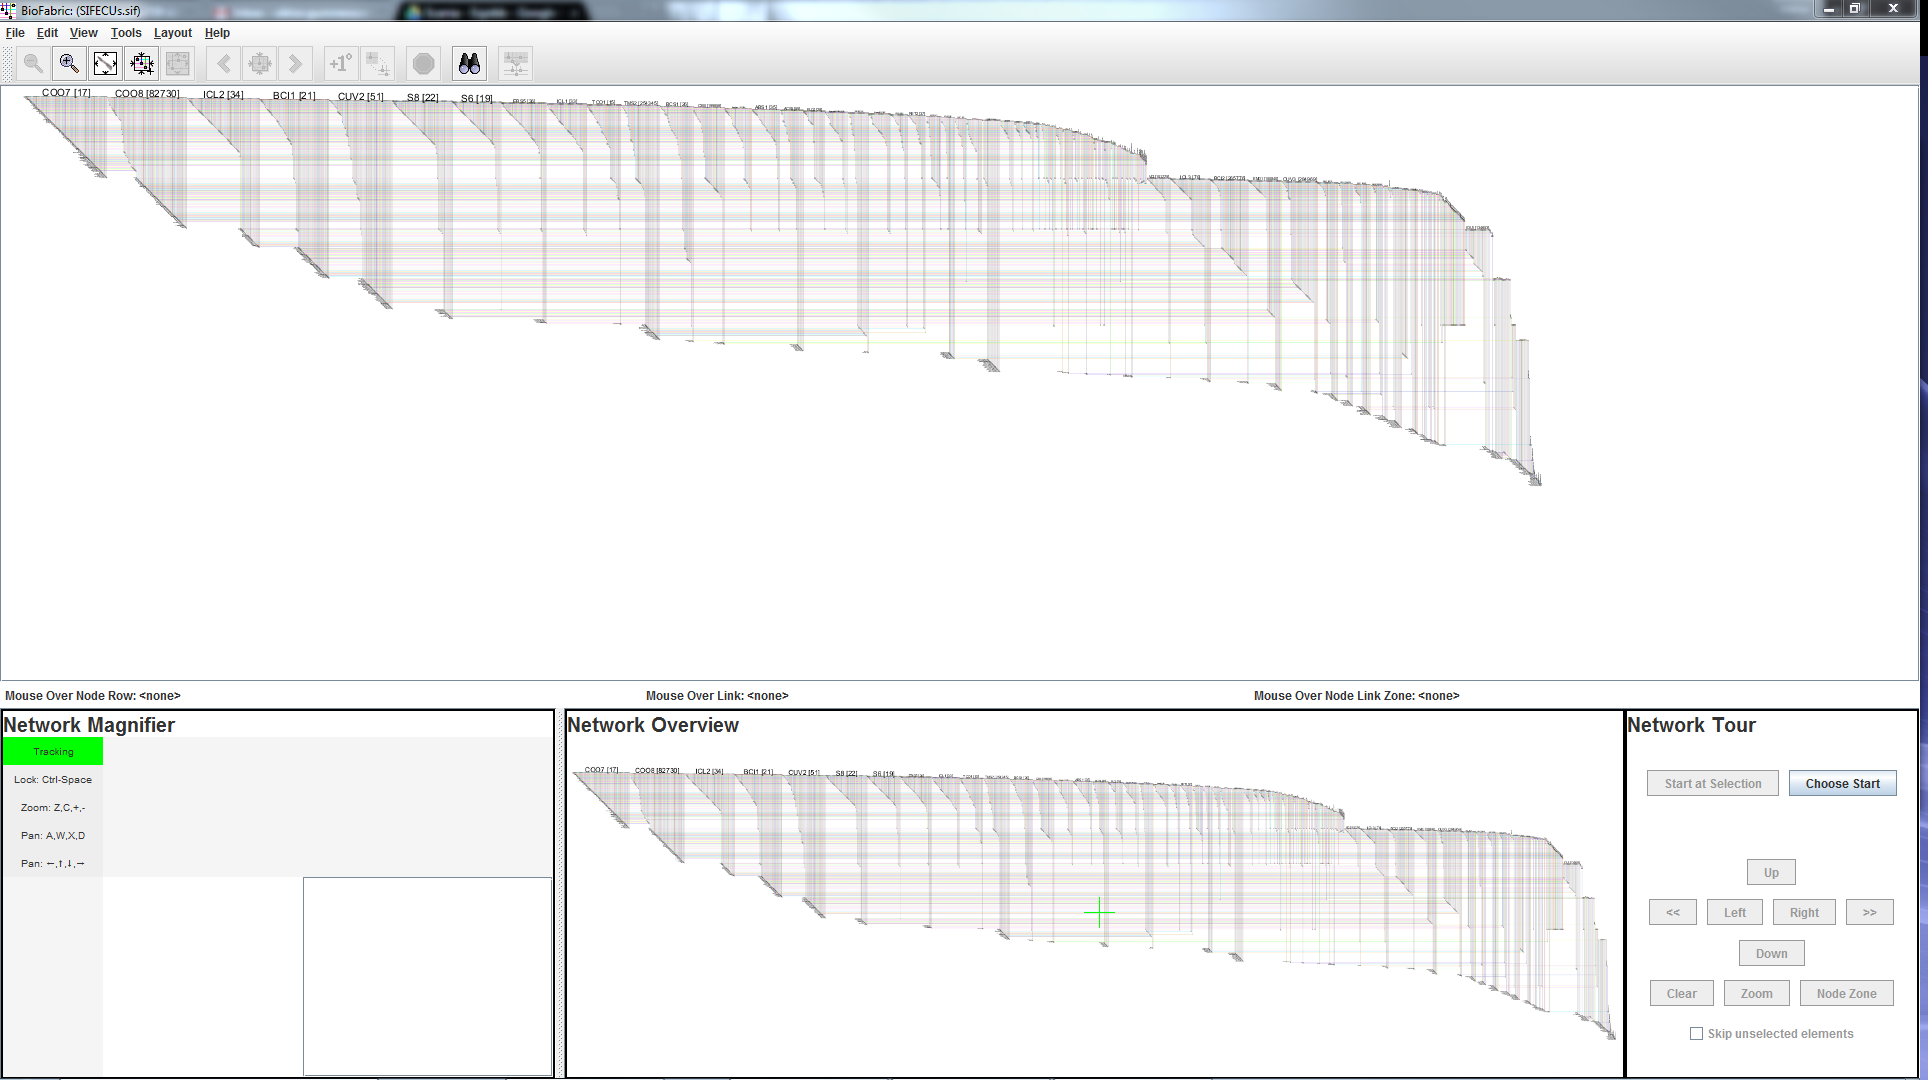
\includegraphics[scale=0.3]{SesammVisualAppPics/BioFabric/Undirected/ECU/AllaECU1}
	\caption{An overview of a network using the BioFabric view were all ECUs were chosen.}
	\label{fig:AllaECU1BIO}
\end{figure}

 \newpage
\begin{figure}[!htbp]
	\centering
	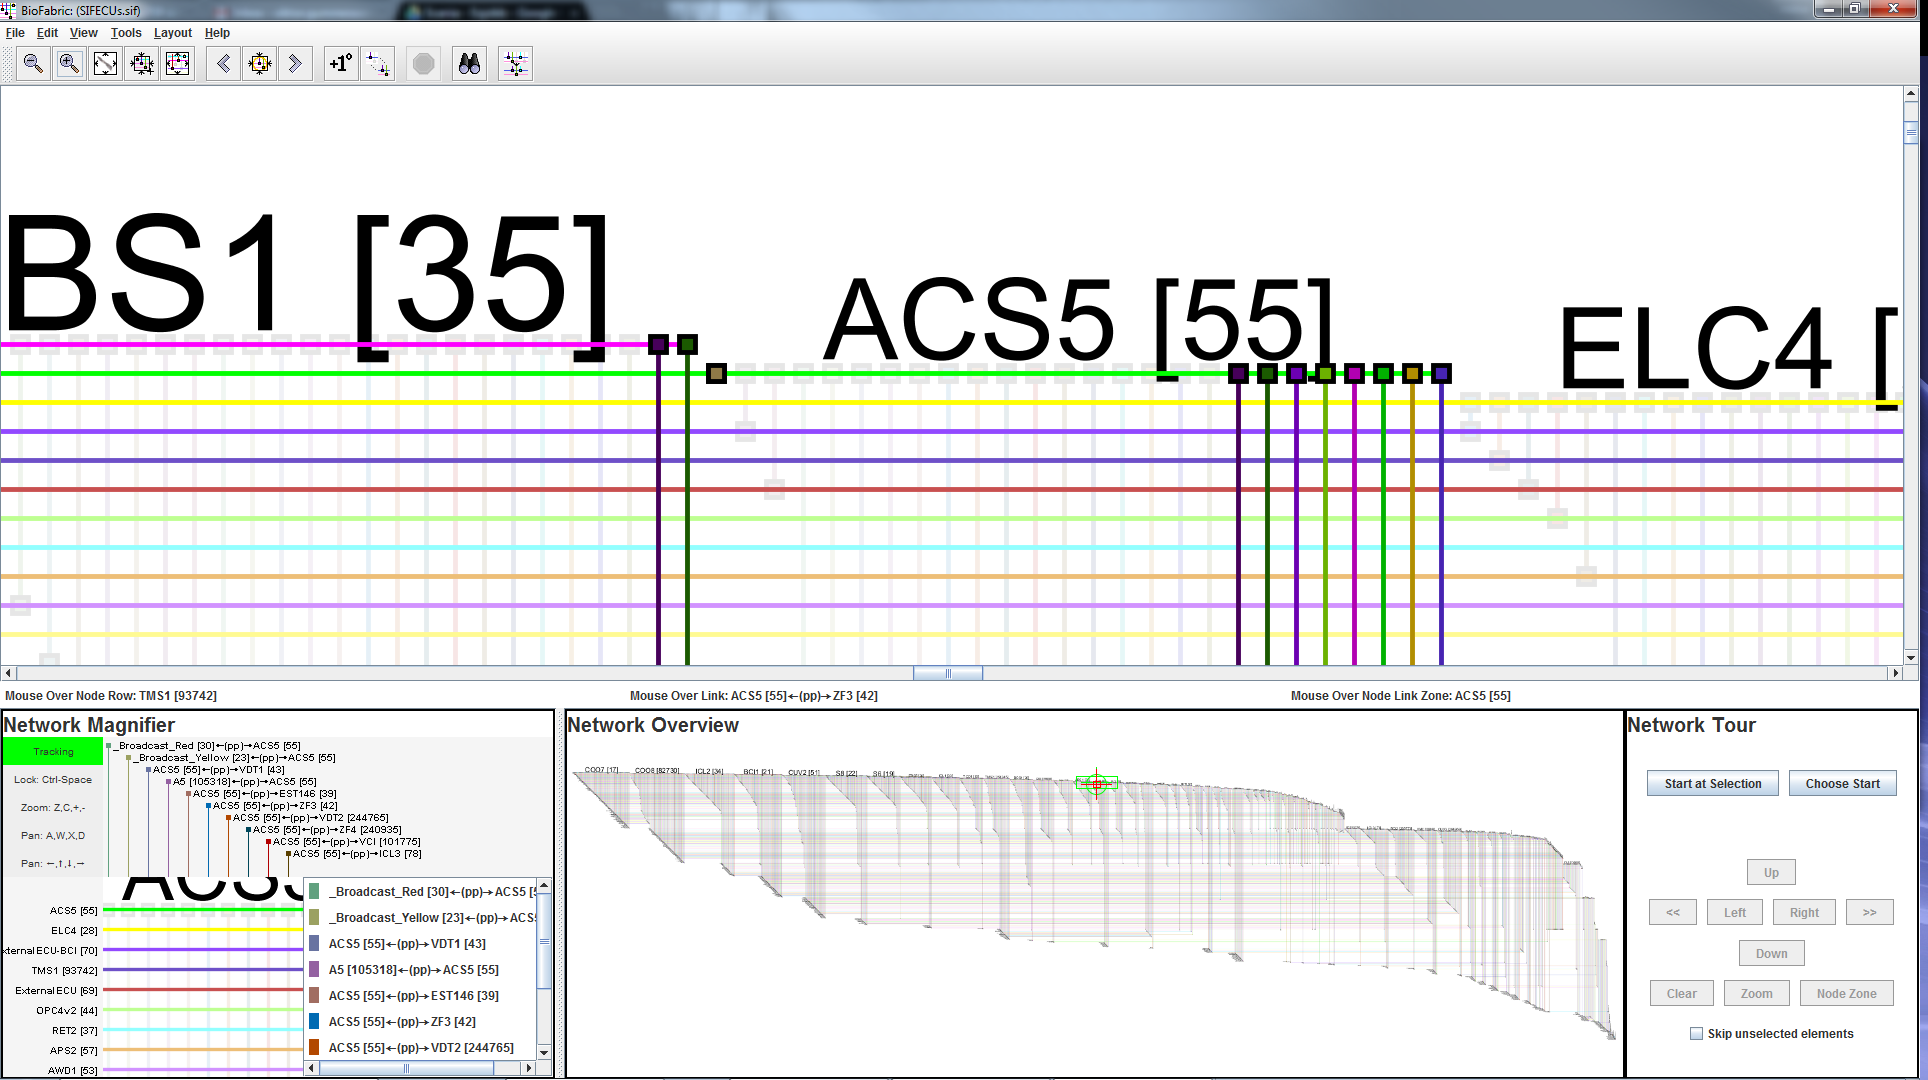
\includegraphics[scale=0.3]{SesammVisualAppPics/BioFabric/Undirected/ECU/AllaECU2}
	\caption{Same network as in \ref{fig:AllaECU1BIO} after zooming and selection actions were preformed.}
	\label{fig:AllaECU2BIO}
\end{figure}

\begin{figure}[!htbp]
	\centering
	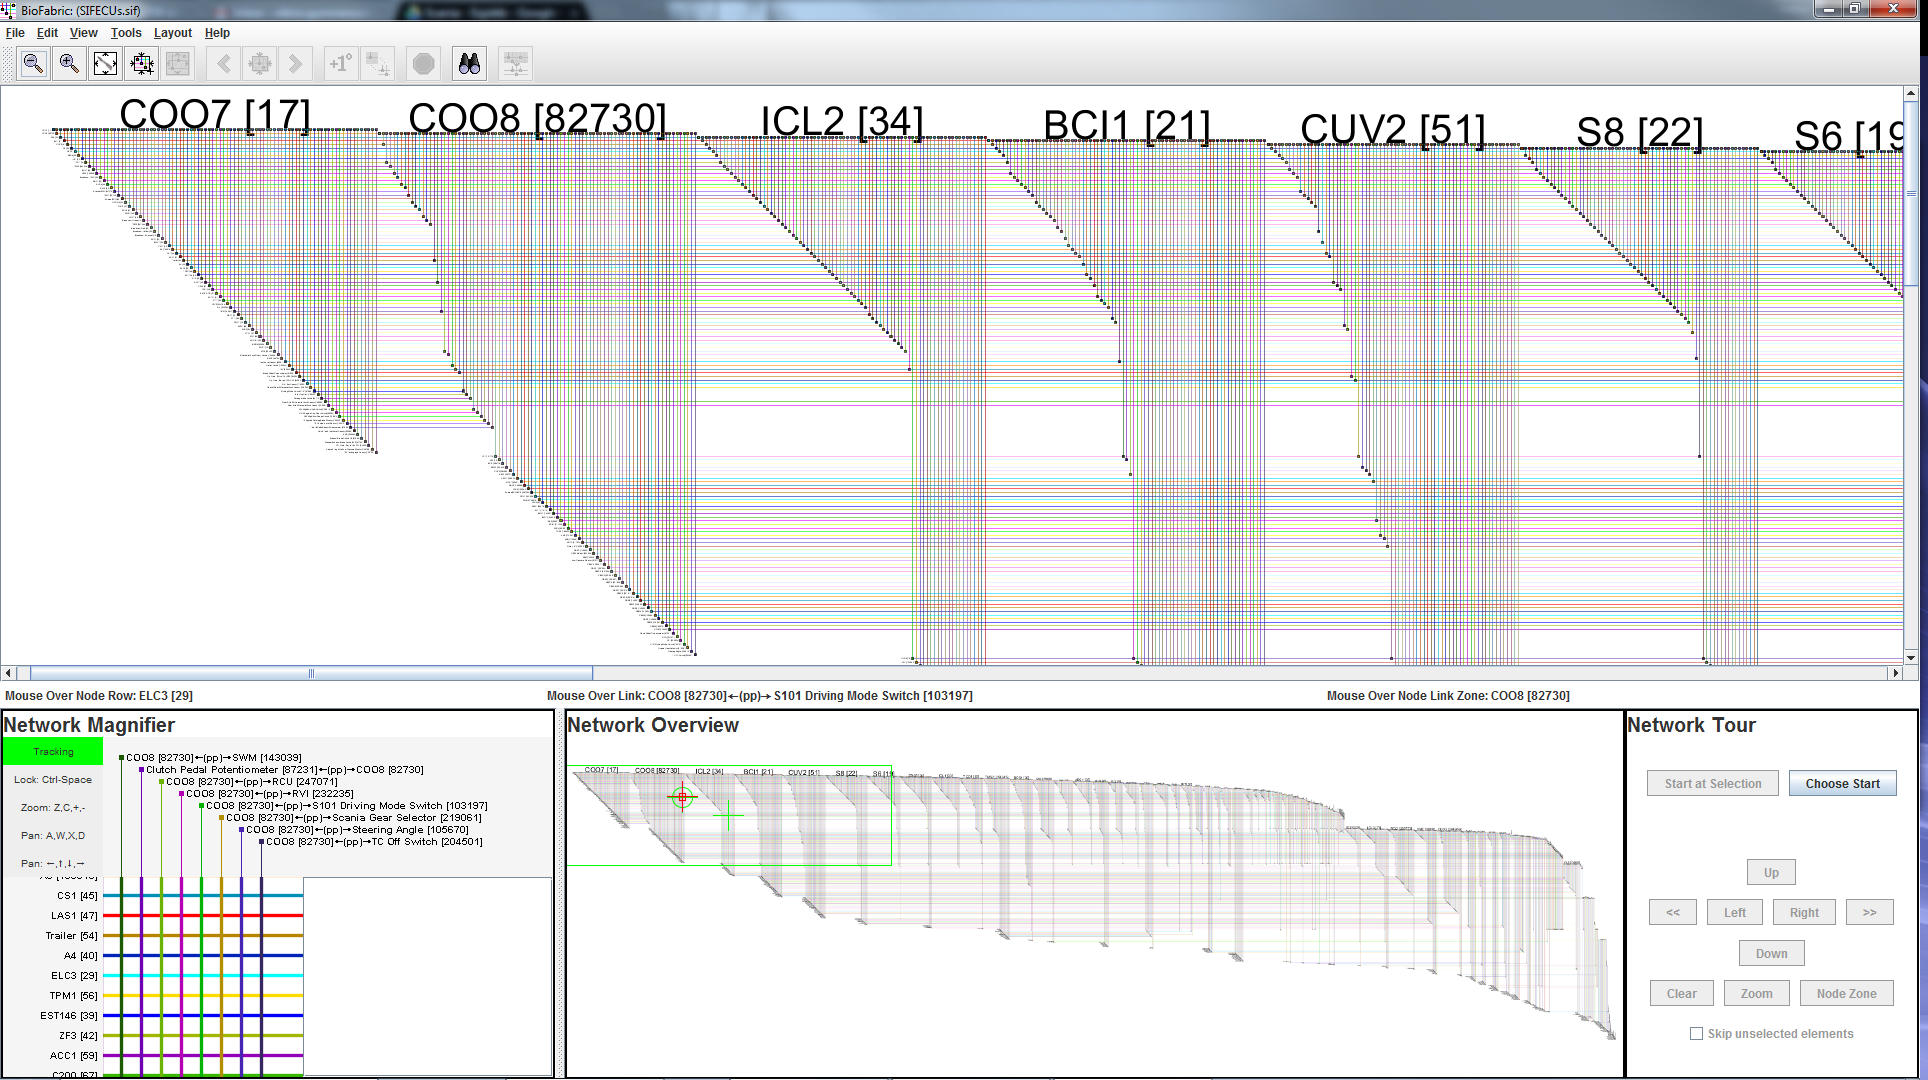
\includegraphics[scale=0.3]{SesammVisualAppPics/BioFabric/Undirected/ECU/AllaECU3}
	\caption{Another example of a selection within the network.}
	\label{fig:AllaECU3BIO}
\end{figure}
 
 \subsubsection{Labeling}
BioFabric also uses a weighted label solution. Here the vertices with highest degree, as in BioFabric becomes the horizontal lines at the top of the view, will be of the greatest size.  
In figure \ref{fig:AllaECU1BIO} one can see this clearly. The reason behind weighting labels becomes fairly obvious when one
starts to think about how it would turn out if BioFabric would try to show all their labels of all vertices at the same 
size. There would be so many labels occluding each other that one would not be able to distinguish which label
belongs to which vertice. Furthermore most part of the graph would have labels occluding each other, making it
difficult to see what label says what.
\subsubsection{Navigation - Situational awareness}
BioFabric's approach is to have more active views in their application at the same time, they have three different views. One main 
view of the network, a second view that gives an overview of the network and show selections made and a third view called the network magnifier. The network 
magnifier displays a sub selection of the network made by the user (a selection) where the user can see all the labels and
connections of vertices in their selection. Figure \ref{fig:AllaECU3BIO} shows all three views where an selection has been made. 

Having these different views, especially the relation between the overview and  network magnifier, tries to 
help toward good situational awareness. The user can get a more detailed view of a subpart of a network using the network magnifier while trying to maintain a global 
context by simultaneously looking at the network overview and main view. 

Having this setup one can argue that their approach goes toward data on demand. Requiring the user 
to have good knowledge about the network being displayed but also to have a good idea of the where and how the
information searched is localized. Putting the pressure on the user to have a good situational 
awareness orientation beforehand, which is not always the case.
 
\subsection{Three-dimensional view - GerbilSphere}
The direction many new visualisation techniques are taking is attempting to take advantage of the extra space in the three-dimensional space. And thus it is of significance for this thesis to incorporate a 
tree-dimensional visualisation technique. Many of these tree-dimensional techniques uses a sphere shape to visualize networks in/on. And it is common that they use some sort of force-directed algorithm
to layout the vertices and edges in this spherical space.

For this application a tree-dimensional view with a layout method that uses the spherical space was used. The view is based on GerbilSphere \cite{Shelley20121016} where the vertices of a network are laid out
 on the surface of a sphere and one navigates from a point of view inside the sphere (though one can zoom out to see the sphere from the outside). For more details about GerbilSpheer see chapter \ref{Theory}
 section \ref{Gerbil:chap2}. Figure \ref{fig:AllaAE1SPW} and \ref{fig:AllaAE2SPW} show the view in use zoomed outside the sphere while Figure \ref{fig:AllaAE3SPW} shows the view from inside the sphere.

\begin{figure}[!htbp]
	\centering
	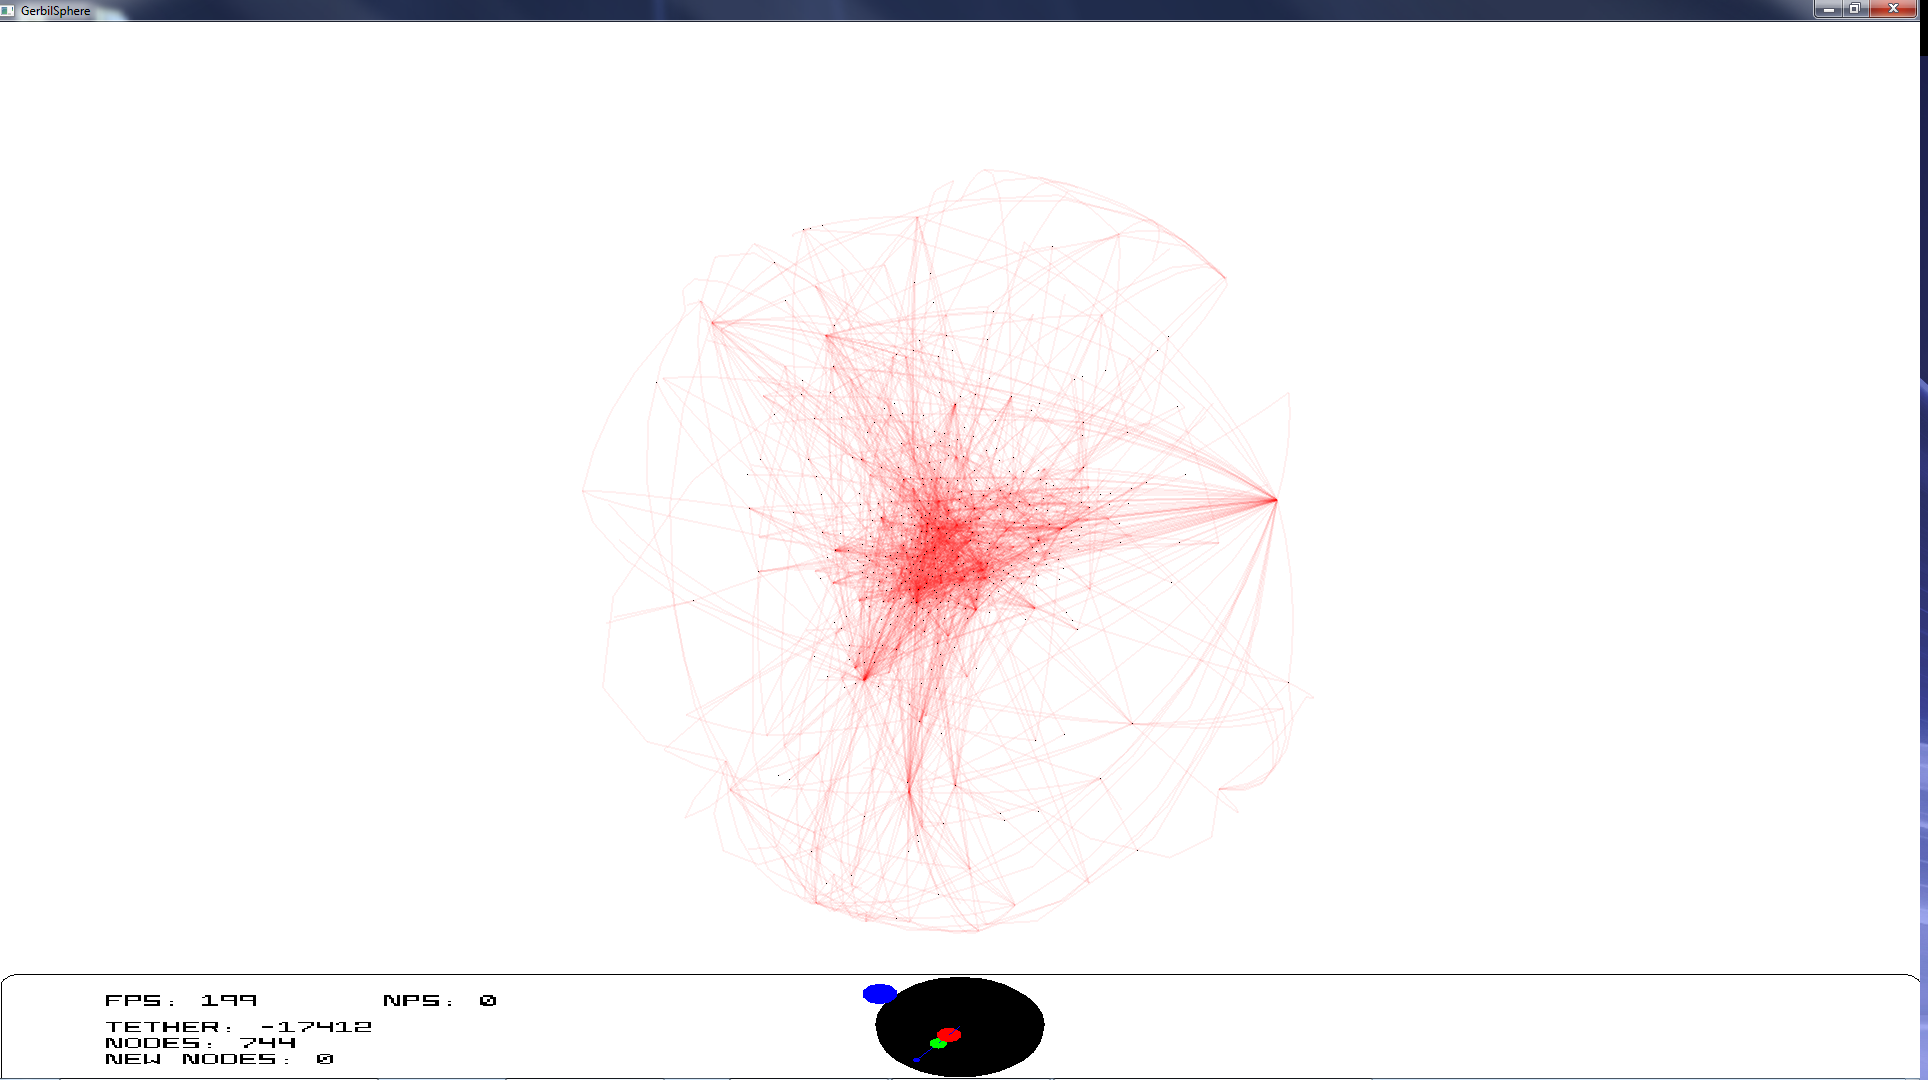
\includegraphics[scale=0.3]{SesammVisualAppPics/SphericalView/AE/AE1}
	\caption{An overview with GirbilSphere of a network were all AEs were chosen.}
	\label{fig:AllaAE1SPW}
\end{figure}

\begin{figure}[!htbp]
	\centering
	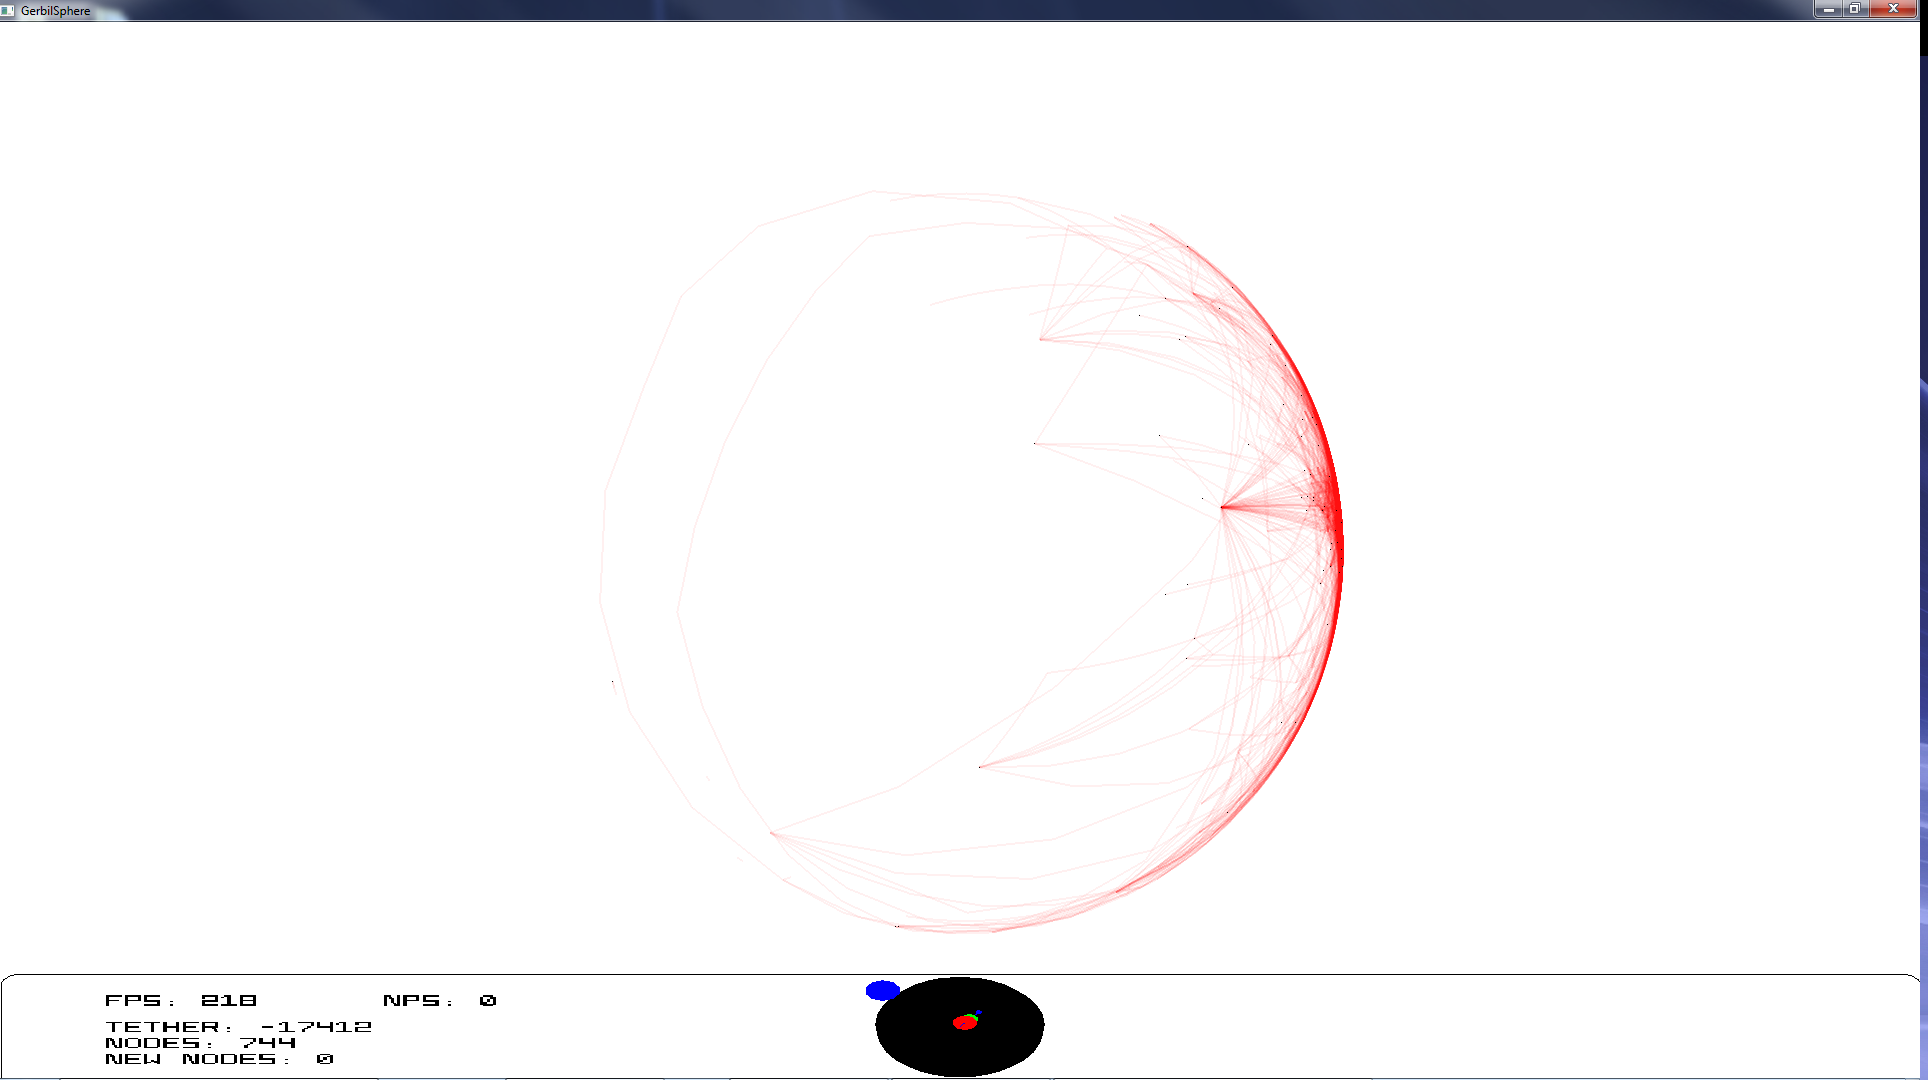
\includegraphics[scale=0.3]{SesammVisualAppPics/SphericalView/AE/AE2}
	\caption{Same network as in figure \ref{fig:AllaAE1SPW} rotated ninety degrees.}
	\label{fig:AllaAE2SPW}
\end{figure}

\begin{figure}[!htbp]
	\centering
	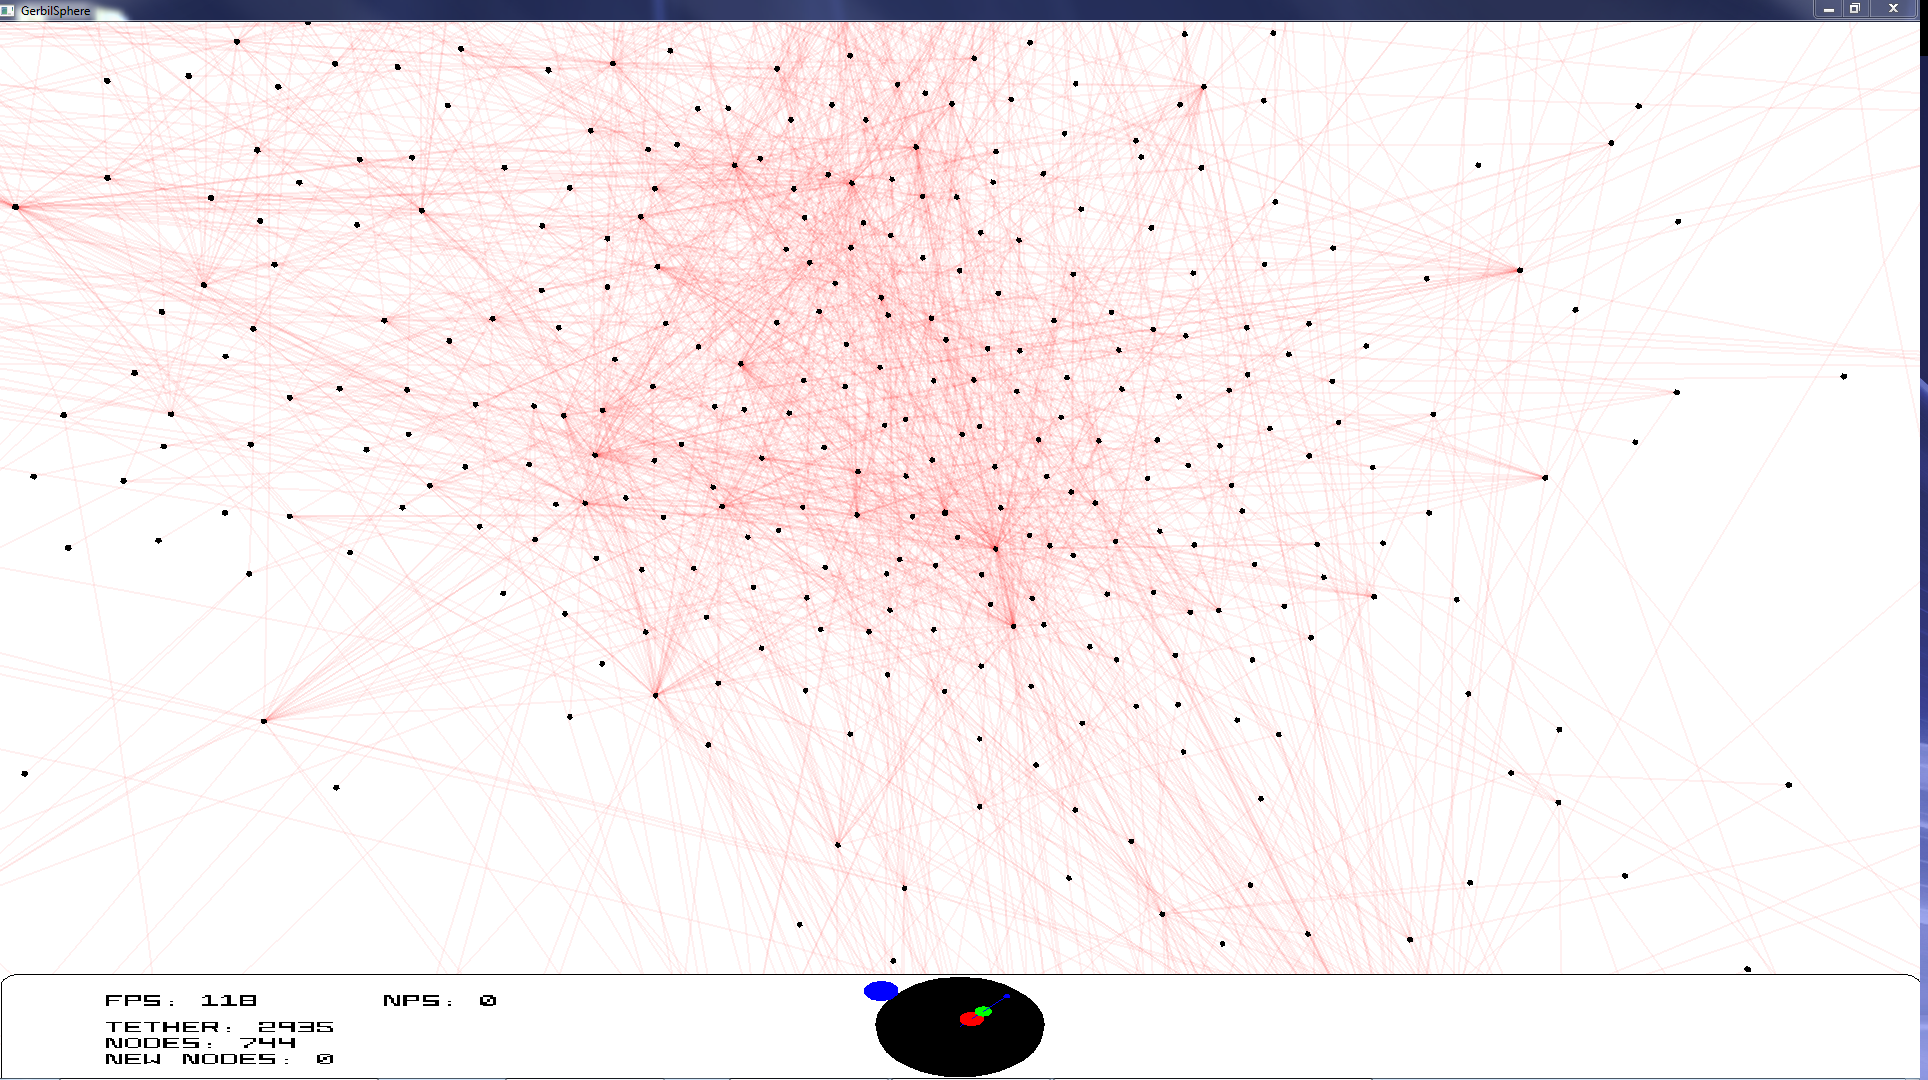
\includegraphics[scale=0.3]{SesammVisualAppPics/SphericalView/AE/AE5}
	\caption{View of the network in figre \ref{fig:AllaAE1SPW} and \ref{fig:AllaAE2SPW} from inside of the sphere.}
	\label{fig:AllaAE3SPW}
\end{figure}
\newpage
\subsubsection{Labeling}
The greatest advantage to this approach is the extra space one gains by using the hyperbolic space. So one might be enticed to draw the conclusion that this is all beneficial thinking,
haveing more space for both labels and vertices lets the application lay out all data points in a satisfactory way. While the fact about more space might be true one will soon see that
obscuration of data becomes a much more severe problem compared to two-dimensional soutions. Now labels and vertices can be obscuring each other in a wider range, laying in front or behind each other.
 
Presumably GerbilSphereAlpha have attempted to work around obscurance taken a information on demand approach. Choosing not to display labels on the
sphere and instead having a separate window that displays information about a vertice when that specific vertice is chosen by the user.
This results in a lower risk of obscuration of labels but at the same time demands more from the user. More in the
sense that the user needs to have a greater knowledge about the network and its structure before hand to be able
to navigate and retrieve desirable data from the visualized network. It also causes a delay in identifying 
vertices when a user needs to click a specific vertice to get information about it. Finally a user might loose orientation
if the user forgets which vertice the user clicked to get information about in previous steps.
\subsubsection{Navigation - Situational awarness}
It has already been indicated that drawing networks in the hyperbolic space offers more space compared to the
two-dimensional space, which is a positive thing. Though this comes with a price, which has to be paid by the end user with a
worsened sense of situational awareness. Due to the the fact that with more space and axis to navigate through it becomes more difficult to keep orientation.
For example a user might take too large of a step in the sphere, loosing track of where the user came from which might result in forcing the user to go further back
or even start over in the task currently being performed.

This becomes a problematic downside when going from a two-dimensional - to a three-dimensional space view, and it needs to be considered and handled. 
GerbilSphereAlpha tries to solve this by using a developed navigation feature that is displayed at the
bottom of the sphere. See \cite{Shelley20121016} for further details. This navigation feature becomes a good first step in 
trying to help the situational awareness of a user, though it is not too intuitive to use at first and it takes some practice to become familiar with.

Going over to the hyperbolic space with a need for more space, having larger networks to display, can reult in a large number of small vertices being displayed.
Which when seeking individual vertices can become infeasable.
Also worth mentioning is that while the hyperbolic space provide more space which is good for larger networks it can 
have an negative effect if it is used on smaller networks. Resulting in a small number of vertices on a greater surface that could produce unnessesary long edges and also vertices
may become further apart then necessary.

The following chapter will try to draw conclusions from the material presented in this chapter.
\chapter{Discussion and Conclusions}
\label{chapter:five}
In this chapter plausible conclusions from the studies and results in previous chapter will be discussed to answer this thesis question.
\emph{Which type of visualisation technique is best suited to visualize big and complex networks?}\\

\section{Which type of visualisation technique is then best suited to visualize big and complex networks?}
\label{sec:conclution}
One thing that becomes fairly clear when reading the research from this thesis is that answering this question
is not an easy task. Due to the fact that this thesis does not go through all existing visualisation techniques,
the evidence from this thesis point towards the conclusion that there is no correct solution answering this
question. It points more towards that there are no best choice of technique to display a complex network that is
independent from the kind of and form of data being used.

It boils down to that when one wants to visualize a complex network one must consider all the features and demands
that the given network needs. Do we need more space for the data? A clean and clear structural way of traversing the network?
How does the need for labeling our vertices look? Do we need to find out how subnetworks looks like or get more information 
about specific vertices and connections? And so on. There exists an indefinite number of different complex networks
and one can not find a generalisation saying that one visualisation technique satisfies all the needs of all networks and 
displays them in an optimal way.

Instead one needs to tailor a specified solution for a specific network and the accompanied requirements of visualisation with it. One needs to 
become very familiar with the data that is going to be displayed along with getting an excellent knowledge of the visualisation needs for the specific
 application. Then use this knowledge to develop features that comply with these needs. Features such as complex filters that
 trims the network to specific data, search functions, highlights etc. It all boils down too the needs of the 
 specific application.
 
 For further research one could be interested in seeing how these different visualisation approaches would 
 cooperate. To see how one use situational awareness is affected by navigating through one view and seeing
 at the same time that change in the different views. How it would affect if one take a sub-selection of 
 a network in one view and see the same sub-selection marked in the other views simultaneously.

\begin{appendices}
\chapter{GraphElement}
\label{Appendix:GraphElement}
\begin{lstlisting}
using System;
using System.Collections.Generic;
using System.Linq;
using System.Text;
using System.Threading.Tasks;

    public class GraphElement : IEquatable<GraphElement>
    {
         * */
        private string name;

        /* id that is a sequiental id, 0,1,2... and so on
         * Needed because some datastructures requers the 
         * elements to have ids on this form.
         * */
        private int internalID;
        //Actual id taken from database.
        private int elementID;

        //Constructor that sets the name and internal id.
        public GraphElement(string name, int id)
        {
            this.name = name;
            this.elementID = id;
        }

        public override int GetHashCode()
        {
            return elementID.GetHashCode();
        }

        //Return name of GraphElement.
        public string GetName()
        {
            return name;
        }

        //Return internal sequential id of GraphElement.
        public int GetInternalID()
        {
            return internalID;
        }

        //Return internal id of GraphElement.
        public int GetElementID()
        {
            return elementID;
        }

        //Set the internal id of GraphElement.
        public void SetInternalID(int newID)
        {
            internalID = newID;
        }

        /*
         * Methods used for commpareing two GraphElements
         * */
        public bool Equals(GraphElement element)
        {
            return elementID == element.elementID;
        }

        public override bool Equals(object obj)
        {
            GraphElement element = (GraphElement)obj;
            return elementID == element.elementID;
        }
    }

\end{lstlisting}
\chapter{Parsers}
\label{Appendix:Parser}
\begin{lstlisting}
using System;
using System.Collections.Generic;
using System.Linq;
using System.Text;
using System.Threading.Tasks;
using System.IO;

namespace GraphParser
{
    public class graph
    {
		//Dictionary for VTK evaluation
        public Dictionary<int,LinkedList<int>> vtkDic;

		//Method to read a graph from given file, path. 
        private Dictionary<int, LinkedList<int>> readGraph(String path)
        {
            string edge;
            vtkDic = new Dictionary<int, LinkedList<int>>();
            try
            {
                using (StreamReader sr = new StreamReader(path))
                {
                    int? nrNodes = convertString(sr.ReadLine());
                    for (int i = 0; i < nrNodes; i++)
                    {
                        int id = i + 1;
                        vtkDic.Add(id, new LinkedList<int>());
                    }

                        while ((edge = sr.ReadLine()) != null)
                        {
                            string[] edges = edge.Split(',');
                            int? source;
                            int? sink;
                            if ((source = convertString(edges[0])) != null && (sink = convertString(edges[1])) != null)
                            {
                                LinkedList<int> getEdges = vtkDic[(int)source];
                                getEdges.AddLast((int)sink);
                                vtkDic[(int)source] = getEdges;
                            }
                        }
                }
            }
            catch(Exception e) 
            {
                Console.WriteLine("File could not be read:");
                Console.WriteLine(e.Message);
            }
            return vtkDic;
        }
		
		//Helpmethod to convert a string to an int
        private int? convertString(string obj) 
        {
            int? numVal;
            try
            {
                numVal = Convert.ToInt32(obj);
            }
            catch (FormatException e)
            {
                Console.WriteLine("Input string is not a sequence of digits.");
                numVal = null;
            }
            catch (OverflowException e)
            {
                Console.WriteLine("The number cannot fit in an Int32.");
                numVal = null;
            }
            return numVal;
        }
		//Get method for dictionary.
        public Dictionary<int,LinkedList<int>> dictionary
        {
            get
            {
                return vtkDic;
            }
        }

		//Get method for size of dictionary.
        public int size
        {
            get
            {
                return vtkDic.Keys.Count;
            }
        }

		//Method for use at evaluation of libraries. Get a test graph of size of vertices 50, 100, 500 or 1000.
        public Dictionary<int, LinkedList<int>> getGraph(int size)
        {
            switch (size)
            {
                case 50:
                    return readGraph("C:/Users/VGUXT8/Documents/VisualizeSystem/Performance review of libraries/Data/50_Nodes.txt");
                case 100:
                    return readGraph("C:/Users/VGUXT8/Documents/VisualizeSystem/Performance review of libraries/Data/100_Nodes.txt");
                case 500:
                    return readGraph("C:/Users/VGUXT8/Documents/VisualizeSystem/Performance review of libraries/Data/500_Nodes.txt");
                case 1000:
                    return readGraph("C:/Users/VGUXT8/Documents/VisualizeSystem/Performance review of libraries/Data/1000_Nodes.txt");
                default:
                    return null;
            }
        }
		
		//GML Parser
        public void To_graphMl(StreamWriter writer, Dictionary<GraphElement, LinkedList<GraphElement>> GraphData)
        {
            writer.WriteLine("<?xml version=\"1.0\" encoding=\"UTF-8\"?>");
            writer.WriteLine("<graphml xmlns=\"http://graphml.graphdrawing.org/xmlns\"");
            writer.WriteLine("    xmlns:xsi=\"http://www.w3.org/2001/XMLSchema-instance\"");
            writer.WriteLine("    xsi:schemaLocation=\"http://graphml.graphdrawing.org/xmlns");
            writer.WriteLine("      http://graphml.graphdrawing.org/xmlns/1.0/graphml.xsd\">");
            writer.WriteLine("  <graph id=\"G\" edgedefault=\"undirected\">");
			
            foreach (var key in GraphData.Keys)
            {
                writer.WriteLine("    <node id=\"n" + key.GetInternalID() + "\"/>");
            }
            foreach (var key in GraphData.Keys)
            {
                foreach (var neighbour in GraphData[key])
                {
                    writer.WriteLine("    <edge source=\"n" + key.GetInternalID() + "\" target=\"n" + neighbour.GetInternalID() + "\"/>");
                }
            }

            writer.WriteLine("  </graph>");
            writer.WriteLine("</graphml>");
            writer.Close();
        }

		//GerbilSphereAlpha parser.
        public void To_Pajek(StreamWriter writer, Dictionary<GraphElement, LinkedList<GraphElement>> GraphData)
        {
            writer.WriteLine("*Vertices " + GraphData.Keys.Count);
            foreach(var node in GraphData.Keys)
            {
                writer.WriteLine("  " + (node.GetInternalID()+1) + "  " + "\"" + node.GetName() + "\"");
            }
            writer.WriteLine("*Edges");
            foreach (var node in GraphData.Keys)
            {
                foreach(var to in GraphData[node]) {
                    writer.WriteLine((node.GetInternalID() + 1) + " " + (to.GetInternalID() + 1) + " 1");
                }
            }
            writer.WriteLine();
            writer.Close();
        }

		//BioFabric Parser.
        public void To_SIF(StreamWriter writer, Dictionary<GraphElement, LinkedList<GraphElement>> GraphData)
        {
            foreach (var node in GraphData.Keys)
            {
                foreach (var to in GraphData[node])
                {
                    string nodeName = node.GetName().Replace(System.Environment.NewLine, string.Empty);
                    string toName = to.GetName().Replace(System.Environment.NewLine, string.Empty);
                    writer.WriteLine(nodeName + "\tpp\t" + toName);
                }
            }
            writer.WriteLine();
            writer.Close();
        }
    }
}

\end{lstlisting}
\chapter{Test data}
\begin{tabular}{ l l }
G50: & 50 vertices, 592 edges.\attachfile{50_nodes.txt}\\
G100: & 100 vertices, 3941 edges.\attachfile{100_nodes.txt}\\
G500: & 500 vertices, 99641 edges.\attachfile{500_nodes.txt}\\
G1000: & 1000 vertices, 399969 edges.\attachfile{1000_nodes.txt}\\
\end{tabular}
\label{testdata}

\chapter{Library evaluation}
\label{app:library:evaluation}
\subsection{Libraries of interest}
For the considered libraries of use for the implementation four different categories is used to classify them. Open-source libraries, closed-source libraries, 3D-approaches and non-conventional graph visualisation approaches.
\subsubsection{Open-source libraries}
\textbf{\textit{\underline{QuickGraph}}}\\
\newline
QuickGraph\cite{website:codeplex} is a library containing generic graph data structures and algorithms for a range of graph problems, developed for .Net\cite{website:Dotnet} use. Such as classical problems like maximum flow, topological sort, shortest path, depth search, etc.\
\newline
\\
\textbf{\textit{Supports:\cite{website:quickDoc}}}\
\
\newline
\
\begin{enumerate}
\item{Graph data structures}
	\begin{enumerate}[label*=\arabic*.]
		\item{Directed graph}
		\item{Undirected graph}
		\item{Dense graph}
		\item{Sparse graph}
	\end{enumerate}
\item{Graph computational Algorithms}
	\begin{enumerate}[label*=\arabic*.]
		\item{Topological sort}
		\item{Strongly connected components}
		\item{Minimum spanning tree}
	\end{enumerate}
\end{enumerate}}
\
\textbf{\textit{Notes:}}\
\newline
\\
QuickGraph does not support an option to use an own solution for visualisation of graphs but points to the layout library Graphviz\cite{website:graphviz} that QuickGraph claims work well with their data 
structures\cite{website:quickGGviz}. This applies to layout algorithms as well.\\
\newline
\textbf{\textit{\underline{Graphviz}}}\\
\newline
Graphviz\cite{website:graphviz} - graph visualization software.  Graphviz provides different layout algorithms and take descriptions of graphs in a text language as input. Normal usage with Graphviz is by using DOT (graph description language)\cite{website:wikipediaDOT}. 

It can be used with QuickGraph as a C\# wrapper. Other wrappers for C\# and .Net one could use are graphviznet\cite{website:graphviznet} and graphviz4net\cite{website:graphviz4net}.
\newline
\\
\textbf{\textit{Supports:}}\
\
\newline
\
\begin{enumerate}
	\item{Layout algorithms\cite{website:graphviz}}
	\begin{enumerate}[label*=\arabic*.]
		\item{Dot}
		\item{Neato}
		\item{Fdp}
		\item{Sfdp}
		\item{Twopi}
		\item{Circo}
		\item{Osage}
	\end{enumerate}
\end{enumerate}}
\
\newline
\textbf{\textit{\underline{GraphX}}}\\
\newline
GraphX is an advanced open-source .Net library for graph visualization with capabilities to rend large graphs with large amount of vertices and edges which
depends on the QuickGraph library\cite{website:graphx}. It also uses partial code from Graph\#\cite{website:graphsharp}, WPFExtensions\cite{website:WPFExtensions}, NodeXL\cite{website:NodeXL} and 
Extended WPF Toolkit\cite{website:wpftoolkit}, which are open-source projects. 

It is based on WPF for rendering graphs and can be seen as the successor too Graph\#. GraphX is the new Apache Sparks API for graphs and 
graph-parallel computation. It introduces a new API that operates on both tables and graphs and incorporate this API as a library using graph parallel techniques 
to be as fast as specialized systems (such as GraphLab, Giraph and Pregel). By embedding this graph-parallel model in Spark it enables GraphX to integrate easily with RDDS
(Resilient Distributed Datasets: A Fault-Tolerant Abstraction for In-Memory Cluster Computing) and perform data parallel operation while also enabling the speed of specialize graph systems\cite{website:graphxPG}.\\
\\
\textbf{\textit{Supports:\cite{website:graphx}}}\
\
\newline
\
\begin{enumerate}
	\item{Layout algorithms}
	\begin{enumerate}[label*=\arabic*.]
		\item{BoundedFR (Fruchterman Reingold).}
		\item{Circular.}
		\item{CompoundFDP.}
		\item{EfficientSugiyama.}
		\item{Sugiyama.}
		\item{FR.}
		\item{ISOM.}
		\item{KK (Kamanda and Kawai).}
		\item{LinLog.}
		\item{Tree.}
	\end{enumerate}
	\item{Possibility to implement an own layout algorithm (external layout algorithm).}
	\item{Visual control}
	\begin{enumerate}[label*=\arabic*.]
		\item{Delete animation of vertices and edges.}
		\item{Mouse over control animation}
		\item{Custom animations}
		\item{Highlighting of vertices and edges.}
		\item{Zoom control.}
		\item{Area selection of vertices.}
		\item{Area zooming and smooth animations.}
	\end{enumerate}
\end{enumerate}}
\
\textbf{\textit{Notes:}}\
\newline
\\
There is no documentation of implemented functions for nested graphs. A nested graph is a graph were vertices can contain subgraphs within themselves.\\
\newline
\textbf{\textit{\underline{MSAGL}}}\\
\newline
MSAGL\cite{website:MSAGL}, Microsoft Automatic Graph Layout, is a .Net tool for graph layout and viewing. It is built on the Sugiyama scheme\cite{website:SugiyamaWiki} that produce hierarchical layouts. Where the 
vertices are drawn in horizontal layers and the edges are often drawn in a downward fashion between vertices. MSAGL contains its own layout engine.
\newline
\\
\textbf{\textit{Supports:\cite{website:MSAGL}}}\
\
\newline
\
\begin{enumerate}
\item{Layout algorithms.}
	\begin{enumerate}[label*=\arabic*.]
		\item{Sugiyama.}
	\end{enumerate}
\item{Editable layout after initial layout.}
\item{Navigation of graph}
	\begin{enumerate}[label*=\arabic*.]
		\item{Zoom.}
		\item{Pan.}
		\item{Search and focus function.}
	\end{enumerate}
\item{Visual control.}
	\begin{enumerate}[label*=\arabic*.]
		\item{Highlighting of vertices.}
		\item{Zoom.}
	\end{enumerate}
\end{enumerate}}
\
\subsubsection{Closed-source libraries}
\newline
\textbf{\textit{\underline{yFiles(yWorks)}}}\\
\newline
yFiles\cite{website:yFiles} provides data structures and algorithms for graph operations. Including automatically layouts for graphs and visualization
 controls for those graphs. yFiles are supported for different platforms, including .Net where one can either use a library for Windows Forms\cite{website:WindowsForms}, WPF\cite{website:WPF} or Silverlight\cite{website:Silverlight}. \\
\\
\textbf{\textit{Supports:\cite{website:yFilesDotNet}\cite{website:yFilesWPF}\cite{website:yFilesSilverlight}}\
\
\newline
\
\begin{enumerate}
	\item{Layout algorithms}
	\begin{enumerate}[label*=\arabic*.]
		\item{Circular layout.}
		\item{Hierarchical layout.}
		\item{Organic layout.}
		\item{Orthogonal layout.}
		\item{Tree layout.}
		\item{Incremental layout.}
	\end{enumerate}
\item{Edge routing algorithms.}
	\begin{enumerate}[label*=\arabic*.]
		\item{Organic routing.}
		\item{Orthogonal routing.}
	\end{enumerate}
\item{Visual control.}
	\begin{enumerate}[label*=\arabic*.]
		\item{Highlighting controls.}
		\item{Zoom.}
		\item{Smooth change animations.}
	\end{enumerate}
\end{enumerate}}
\
\textbf{\textit{Notes:}}\
\newline
\\
yFiles also supports incremental layout, meaning that when a graph needs to be updated (addition/removal of vertices or edges) the whole graph is not re-computed but tries to maintain as much as possible
 of the same layout as before. Also yFiles tries to supports nested graphs, but has some restrains on the data to be able to use it. Their function is called collapsible tree, which requires the data to
 be able to be structured as a tree.
\
\subsubsection{An comparison of given libraries.}
\
\textbf{\textit{Attribute matrix:}}\
\newline
\\
The following matrix, Figure \ref{fig:libAttributeMatrix:appendix}, lists important functionality one looks for when considering a programming library for implementing visualisation methods. The matrix gives an overview of what the 
different libraries supports from the start. This matrix helps as a basis when selecting libraries for the implementation.\\

\begin{figure}[!htbp]
	\centering
	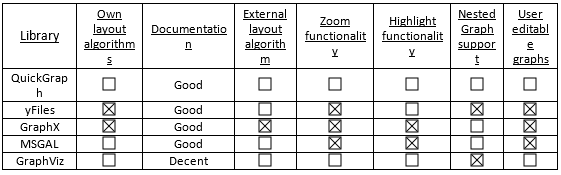
\includegraphics[scale=1.0]{LibraryAttributeMatrix}
	\caption{Attribute matrix}
	\label{fig:libAttributeMatrix:appendix}
\end{figure}
\\
\subsubsection{3D approaches}\\
\\
\newline
\textbf{\textit{\underline{Libraries}}}\\
\newline
For developing advanced 3D graphics the two most common approaches is to use either OpenGL\cite{website:OpenGL} or Direct3D\cite{website:Direct3D}. To use OpenGL in windows one has a few options, one can for example use
 OpenTK that wraps OpenGL, OpenCL\cite{website:OpenCL} and OpenAL\cite{website:OpenAL}. 

Direct3D is part of the DirectX API that uses hardware acceleration (if available on the graphics card).
\\
\subsubsection{Differences between OpenGL and Direct3D}\\
\newline
OpenGL is being developed largely by a consortium of different parties and follows a largely open standard. While Direct3D are being developed 
and maintained by Microsoft and is completely proprietary in its implementation. Resulting in a big platform difference, where OpenGL is supported on a wide range of platforms and languages,
while Direct3D is bound to Microsoft Windows systems. 

At last there are different methods used to introduce new hardware and features. OpenGL do this by allowing hardware manufactures 
to be able to implement special functions, called extensions that give immediate access to features of new hardware. As for Direct3D,  Microsoft needs to process theses features and then release 
access to these in forms of new functions. Here OpenGL allows new features to be accessible quicker then Direct3D, though reduces the overall compatibility of a program using the extensions. 
And the other way around, Direct3D takes longer to give access to the new features but compatibility across different systems is being maintained.

The aspect of hardware managing differs in these two libraries.
OpenGL hides the hardware and works so that the implementation handles hardware resources, users of OpenGL use functions for drawing which relies on drivers to directly access the hardware. Direct3D on
the other hand lets the application handle the hardware resources. With OpenGL it becomes easier to write applications but hard to see the status of hardware resources and
thus must hope that the implementation uses the resources in a way that suits the related application. While with Direct3D the writing of the application may be more complex but have the possibility to use 
hardware resources in the most efficient way for the application.\cite{website:wisegeek}

Both these differs a bit form previous discussed libraries in the sense that there are no (known) support for graph visualization. 
So for instance no layout algorithms for graphs like force directed or data structures to represent a graph. This implies that all has to be implemented from scratch, taking more time but open
up for less restrictions on what one can do.\\
\newline
\textbf{\textit{\underline{VTK}}}\\
\newline
VTK (Visualization Toolkit)\cite{website:vtk} is an open-source software system for 3D computer graphics, image processing and visualization. At its core VTK is implemented as a C++ toolkit and it supports parallel
 processing which help in performance. VTK is a popular library when it comes to visualize scientific data, which is often big and complex. 
 
There are a number of wrapper languages making it possible in addition to C++ use VTK through for instance  Python, Java and .NET.\\
\subsubsection{Non conventional graph visualization approaches}\\
When it comes to the visualisation techniques like BioFabric, Hive Plots and Treemap (described in chapter \ref{Theory}) there are few libraries that support this compared to the amount of libraries there are
 to visualize the classical node/edge graphs. How these approaches can be used are shown below.\\
\newline
\textbf{\textit{\underline{BioFabric:}}}\\
\newline
BioFabric has one release which is an open-source Java application with some documentation that can be found at\cite{website:biofabricdoc}. Though BioFabric is built on a relatively easy and intuitive algorithm, one could
 take the option of implementing an own version. Having their own customized features that suits one's purpose.\\
\newline
\textbf{\textit{\underline{Hive Plots:}}}\\
\newline
For hive plots there are some choices, one used is a Java based library\cite{website:JHive}. There are also libraries for R\cite{website:R}, HiveR\cite{website:HiveR}, that supports hive plots in the two dimensional and three dimensional space.
The framework D3.JS\cite{website:D3JS} is an other option that is a JavaScript to create hive plots. And pyveplot\cite{website:pyveplot} that is a library for hiveplots in Python\cite{website:python}.\\
\newline
\textbf{\textit{\underline{Tree Map:}}}\\
\newline
As for Treemaps there are some choices as well. For .Net, which is this thesis working environment, there is the WPF Treemaps \& SquarifiedTreeMaps control library\cite{website:WPFTreeMaps}, though it has poor documentation.
 Another alternative is the .NET Treemap Control library\cite{website:devxTreeMap}. Again the problem lies in little documentation and it is hard to get information about the library when this was part of an old Microsoft
 research project called Netscan.\\
\newline
\textbf{\textit{\underline{GerbilSphere:}}}\\
\newline
GerbilSphere visualize graphs by projecting nodes and edges to the surface of a sphere, defined as an inner sphere 2D system. It differs from other graph visualisation techniques that also uses spheres
in the way that in GerbilSphere the observers point of view is from inside the sphere.

GerbilSphere is an open source project. No API is available, though good documentation is presented within the code.\\
\\
\textbf{\textit{Supports:\cite{Shelley20121016}}}\
\
\newline
\
\begin{enumerate}
	\item{Specialised layout algorithm that is based on force-directed algorithms.}
	\begin{enumerate}[label*=\arabic*.]
		\item{Static layout when adding/removing nodes.}
	\end{enumerate}
\item{Labelling.}
\item{Menus when choosing specific nodes.}
\item{Visual control.}
	\begin{enumerate}[label*=\arabic*.]
		\item{Zoom.}
		\item{Paning.}
		\item{Fisheye view.}
		\item{Variablezoom.}
	\end{enumerate}
\end{enumerate}}
\
\textbf{\textit{Notes:}}\
\newline
\\
While GerbilSphere does not support nested graphs this becomes of less interest when the whole graph is being visualized.

\subsection{Library selection for evaluation}
From the matrix in figure \ref{fig:libAttributeMatrix:appendix} one conclude that GraphX and yFiles are two possible candidates for usable libraries. They both support more functionality than QuickGraph, MSGAL and 
GraphViz. Therefore they will be included in the evaluation.

Needed is also an option for implementing three dimensional views. For this purpose the VTK library is included when it has support for graph visualization.
\subsection{Test set up}
\label{sec:test:set-up}
The libraries have been tested on two different aspects, rendering speed and smoothness. Rendering speed is measured as the time it takes a specific library to draw up a given graph. As for
smoothness the frames per second (fps) rate has been measured during navigation through corresponding graphs. Navigation actions such as panning and zooming.
\subsubsection{Data}
The data used for these tests has been produced with the use of Gephi\cite{website:gephi}. Four different graphs were created for testing:

\begin{itemize}
	\item{50 vertices with 592 edges. Referred as G50.}
	\item{100 vertices with 3941 edges. Referred as G100.}
	\item{500 vertices with 99641 edges. Referred as G500.}
	\item{1000 vertices with 399969 edges. Referred as G1000.}
\end{itemize}
\newline
Given graphs can be found in appendix \ref{testdata}.
\subsubsection{Hardware}
The evaluations where runned on the same computer for each graph and library with the following hardware:\\
\newline
\begin{tabular}{ l l }
	Processor: & \textcolor{blue}{Intel(R) Core(TM) i5-3470 CPU @ 3.20GHz}\\
	Video Card: & \textcolor{blue}{Intel(R) HD Graphics. 64 MB Dedicated Memory, 1.7 GB Total Memory}\\
	Memory: & \textcolor{blue}{6.1 GB}\\
	Operating System: & \textcolor{blue}{Microsoft Windows 7 Enterprise Edition Service Pack 1 (build 7601), 64-bit}\\
\end{tabular}	
\subsection{Results from library tests}
Two kinds of users need to be considered when talking about the results from the library evaluations. The users that will indirect use the libraries by using an application 
built on these, we will call these users for end users. Second is the kind of user that will use these libraries to build an application for visualisation, we call these users for developer users.

The needs one have on the libraries differs depending on what kind of user one are. For an end user the speed and smoothness are the two things that shows most. Developer users must also take into consideration
what the different libraries supports and not.\\

\label{sec:library:results}
\textbf{\textit{Speed}}\\
\newline
Each graph have been drawn ten times and the arithmetic mean value of the time has been calculated and given as result. Time is displayed on the form of minutes:seconds.\
\newline
\begin{table}[h]
\centering
\caption{Speed results}
\begin{tabular}{|c|l|l|l|l|}
\hline
\multicolumn{1}{|l|}{} & \multicolumn{1}{c|}{\textbf{G50}} & \multicolumn{1}{c|}{\textbf{G100}} & \multicolumn{1}{c|}{\textbf{G500}} & \multicolumn{1}{c|}{\textbf{G1000}} \\ \hline
\textbf{GraphX}        & 00:00.51461281                    & 00:07.41482771                     & 22:33.4573175                      & Out of memory                       \\ \hline
\textbf{VTK}           & 00:00.01546258                    & 00:00.04138581                     & 00:00.88301525                     & 00:03.53977976                      \\ \hline
\textbf{yFiles}        & 00:00.54974544                    & 00:01.68249026                     & 00:49.60542746                     & 12:11.535764772                     \\ \hline
\end{tabular}
\label{table:librarie-speed:appendix}
\end{table}
\newline
Here one can see that the VTK library is far superior to the other libraries, especially on the larger sized graphs. 
On the smallest graphs the difference are not as significant. For the end users the difference on drawing speed on graphs of size with 50 nodes would not be to notable.
Though the developer users might want to take this into consideration. 
On larger than 50 nodes graphs the difference between these libraries shows fairly clear. GraphX drawing speed decreases rapidly and are not able to draw graphs with a size of 1000 vertices with the hardware used.
yFiles do manage to draw this graph, though it took over 12 minutes compared to VTKs 3 seconds.\\

\newline
\textbf{\textit{Smoothness - FPS(Frames per second)}}\\
\newline
There are three fps measurements for each library were panning actions was being
performed. One zoomed out far away, giving an overview of the graph (Z1), one
zoomed in half way to the centre of the graph (Z2) and a third were the user are
zoomed far in to the graph, being able to distinguish between vertices (Z3).\\
\newline
\begin{table}[h]
\centering
\caption{GraphX}
\begin{tabular}{|c|c|c|c|}
\hline
\multicolumn{1}{|l|}{} & \textbf{Z1}    & \textbf{Z2}    & \textbf{Z3}    \\ \hline
\textbf{G50}           & 17 fps         & 23 fps         & 35 fps         \\ \hline
\textbf{G100}          & 1 fps          & 3 fps          & 5 fps          \\ \hline
\textbf{G500}          & Undetectable   & Undetectable   & Undetectable   \\ \hline
\textbf{G1000}         & Non-executable & Non-executable & Non-executable \\ \hline
\end{tabular}
\label{table-graphx:appendix}
\end{table}
\newline
\begin{table}[h]
\centering
\caption{VTK}
\begin{tabular}{|c|c|c|c|}
\hline
\textbf{}      & \textbf{Z1} & \textbf{Z2} & \textbf{Z3} \\ \hline
\textbf{G50}   & 1000 fps    & 1000 fps    & 1000 fps    \\ \hline
\textbf{G100}  & 500 fps     & 500 fps     & 500 fps     \\ \hline
\textbf{G500}  & 35 fps      & 11 fps      & 3 fps       \\ \hline
\textbf{G1000} & 11 fps      & 7 fps       & 2 fps       \\ \hline
\end{tabular}
\label{table-VTK:appendix}
\end{table}
\newline
\begin{table}[h]
\centering
\caption{yFiles}
\begin{tabular}{|c|c|c|c|}
\hline
\textbf{}      & \textbf{Z1}  & \textbf{Z2}  & \textbf{Z3}  \\ \hline
\textbf{G50}   & 22 fps       & 20 fps       & 25 fps       \\ \hline
\textbf{G100}  & 2 fps        & 3 fps        & 5 fps        \\ \hline
\textbf{G500}  & Undetectable & Undetectable & Undetectable \\ \hline
\textbf{G1000} & Undetectable & Undetectable & 2 fps        \\ \hline
\end{tabular}
\label{table-yFiles:appendix}
\end{table}
\newpage
From these tables one can see that GraphX and yFiles perform almost equally, though VTK outperforms both these libraries with quite a larger margin. VTK is also the only one that could detect a readable 
FPS value when maneuvering the largest sized graph. Both GraphX and yFiles displays a better smoothness (higher FPS) at a deeper zoom, which at first can seem a bit strange. 
The reason for this is that once you are zoomed far enough in the graph, you come to a point where there is less nodes and edges to display on the screen then previous zoom
where the low FPS value starts to increase after this point. 

\subsubsection{To take into consideration}
One thing that becomes overlooked when talking about these different libraries is how one wants to draw graphs. For instance if one wants a small or large representation of nodes. If one is planing on just drawing 
smaller graphs with larger nodes one might be fine using yFiles or GraphX. Though if one wants to draw graphs of the larger kind one might be better suited with the VTK library. These aspects will of course affect 
the speed and smoothness when using these libraries. In this study the basic common configuration for each library has been used.

For the end user the speed and smoothness is what becomes of most importance, because that is what they see when using an application. The developer user must of course take this into account when developing an application.
The developer user must also take into consideration what features that the different libraries support.
 
\chapter{Implementation details.}
\label{appendix:implementation:details}

\section{Views}
\subsection{Force-directed(FD) based view}
\label{FD:View:appendix}
This view was implemented using the VTK library for C\# on the basis 
from the evaluation done in section \ref{sec:libperform}.

In this view the user of the application can choose between showing labels and not. The labelling of the vertices in this view are weighted with a weight based on their degree. This in such a way that the higher
 the degree of a vertice, the higher weight that vertices label will be given. Based on the vertices weights, a priority of which labels to be displayed at a certain point in the network are made. Giving vertices
 with higher degree higher priority. This also results in that depending on which zoom level in a network one are, different labels will be prioritised.

 When it comes to the space this view is using, it is actually up to the user to chose. By holding down shift when navigating an network in this view the z-axle becomes fixed, making it appear as a two dimensional view. 
Otherwise it works in the three dimensional space, where one can navigate through the x-, y- and z-axles. This is unique to this view, the next two views works in the two- or three-dimensional space. 

\subsection{Two-dimensional view - BioFabric}
BioFabric is an open-source Java application which makes it applicable to use for this thesis. Though some changes was needed to be done for it to work with our implementation. Changes concerning the code that conducts the where
and how the input of data for the application were made, changes so that BioFabric becomes compatible with our application. Also additions concerning making sure that the data converts to the correct form for BioFabric to handle
 after data had been input where needed. More about this in \ref{Data:Parsers}.

\subsection{Three-dimensional view - GerbilSphere}
GerbilSphere is an open source application developed in C++. Again the data handling needs to be modified to match the form of data input GerbilSphere uses,
again more about this in \ref{Data:Parsers}.

GerbilSphere handles labels a bit differently than previous views. Instead of trying to place visible labels in the spherical space they have taken an information on demand approach, making it up to the user to prompt for 
specific information at need. This by having a secondary window up that keeps track of actions made in the sphere. As when clicking on a specific vertex getting the information (the label) about that vertex showing in 
this window.
\section{Data representation}
In this section we will go over how we have choosen to represent our data that we want to visualise.
\label{Data-Rep}
\subsection{GraphElement}
To be able to represent data in the earlier stages, before displaying any views, a small class called GraphElement was created. This represents, as its name suggests, an element of a graph such as a vertex or
an edge.

The class holds parameters about the name and ids and implements functions making it possible to distinguish between two different GraphElements. See Appendix \ref{Appendix:GraphElement} for the source code.
\subsection{Data representation within application - DataManager}
DataManager is a class developed to do the actual data retrieval from the working database. To represent a graph internal in the application the DataManager class retrieves the data one wants to visualise and creates
 GraphElement objects that are put into an object of the data structure called Dictionary \cite{website:dictionary}. This in such a way that each object (can be seen as a vertice) of a network will be set as a key in the 
 dictionary and have a tied value in form of a list of GraphElements. Thus one can see the dataset as that a given key (vertice) in the dictionary (network) has a corresponding list Y (neighbours). For instance say that
 GraphElement X is a key and are associated to a list Y, then an object y in Y can be seen as that there exists and edge between X and y.

Then when it comes to actually visualise data one needs to convert the data to the appropriate form for the corresponding view. More about this in the next section.
\subsection{Data parsers}
\label{Data:Parsers}
This section will give account for the resulting data parser written for each of the three views. Parser for the VTK library for the force-directed view, a parser for BioFabric and lastly a parser for GerbilSphereALpha.
 The code for the parsers can be find in Appendix \ref{Appendix:Parser}.
\label{section-parsers}
\subsubsection{VTK data parser}
The VTK library uses a straightforward simple way of representing a graph. It works such as first all the vertices are added getting sequential ids starting from 1. Then one can add edges between these by calling a function with parameters
saying between which two vertices the edge connects, using the vertices ids. Making it very compatible with the DataManager class and GraphElement object.

Because VTK represents their data in such a way and one needs to build the data structure in code behind there was no need to implement a parser for VTK. One could simply retain the necessary information from your network
 and use it directly to functions for building graphs in the VTK library. Though a parser was implemented, reading a text file containing information about a network and storing it in a
 dictionary. Much such as in the DataManager class. This parser was implemented for the evaluation stage for the VTK library. Making it possible to take a text file, generated from Gephi as input and returning a 
 dictionary that could then be used to generate a graph with VTK to be evaluated. See appendix \ref{Appendix:Parser} for the source code of the parser.
\subsubsection{BioFabric data parser}
BioFabric supports tab-delimited .sif files \cite{website:biosif} as input, therefore a parser for transforming data from our DataManager class to SIF files were created. A SIF file has the following form:\
\newline
\begin{itemize}
 From vertice name, tab pp (indicating an edge), and tab followed by to vertice name. For example:\
 \newline
 2	pp	4,
\newline
 meaning there exists an edge between vertice 2 and vertice 4.
 \end{itemize}
 \newline
 Where it states vertex name, the information in that field will be what displays in the BioFabric view as the labels. The source code for the parser can be found in appendix \ref{Appendix:Parser}.
\subsubsection{GerbilSphere data parser}
GerbilSphere supports two different file formats as input. First is Pajek\cite{website:gephipajek} and second the Extensible Graph Markup Language (XGMML)\cite{website:xgmml}. Pajek is on a text based format with the file 
extension .Net. Which first states the number of nodes N, followed by N lines with the vertices id and labels. Next comes "*Edges" followed by X lines defining the networks edges. Where you first have the vertice from id
followed by the to vertice id. The edges can also be weighted, in that case a third value with the weight are added. 

In GerbilSphereAlpha these nodes can have attributes such as positioning for the sphere, the file is then called baked. See \cite{Shelley20121016} for further information.

XGMML is based on the Graph Modelling Language, GML, which is a hierarchical ASCII-based file format for describing graphs. Using tags to describing different graph components.
Though both Pajek and XGMML where usable for this thesis application the Pajek format was in the end used.

A parser for both these file formats where created, following the syntax described above. See appendix \ref{Appendix:Parser} for the source code of these parsers.
\end{appendices}

\nocite{*}\\
\bibliographystyle{plain}
\renewcommand{\bibname}{References}
%\bibliography{C:/Users/Viktor\string~1/Documents/GitHub/Exjobbs-rapport/Chap3/refs}
\bibliography{D:/GitHub/Exjobbsrapport-SecondVersion/Exjobbs-rapport/Chap3/refs}
\end{document}
